%!Tex Root = ../Main.tex
% ./Packete_und_Deklarationen.tex
% ./Titlepage.tex
% ./Motivation.tex
% ./Einführung.tex
% ./Implementierung2_Pntr_Array.tex,
% ./Implementierung3_Struct_Derived.tex,
% ./Implementierung4_Fun.tex,
% ./Ergebnisse_und_Ausblick.tex

\chapter{Implementierung}
\label{ch:implementierung}

\section{Lexikalische Analyse}
\subsection{Konkrette Syntax für die Lexikalische Analyse}
\numberwithin{floatgrammar}{section}

\label{sec:lex_analyse_verwendung_von_lark}
% ./concrete_syntax_picoc.lark
\begin{grammar}[Konkrette Syntax der Sprache $L_{PicoC}$ für die Lexikalische Analyse in EBNF, Teil 1][H][gr:concrete_syntax_lex_teil_1]
  \toprule
  \firstcase{COMMENT}{\dq //\dq\enspace /[{\wedge}\backslash n]{*}/\gralt \dq {/*}\dq\enspace  /(.\mid \setminus n)*?/\enspace \dq {*/}\dq }{L\_Comment}
  \firstcase{RETI\_COMMENT.2}{\dq {//}\dq \dq \text{\textvisiblespace} \dq ? \dq \#\dq /[\wedge\backslash n]{*}/}{}
  \midrule
  \firstcase{DIG\_NO\_0}{\dq 1\dq \gralt \dq 2\dq \gralt \dq 3\dq \gralt \dq 4\dq \gralt \dq 5\dq}{L\_Arith}
  \otherform{\dq 6\dq \gralt \dq 7\dq \gralt \dq 8\dq \gralt \dq 9\dq}{}
  \firstcase{DIG\_WITH\_0}{\dq 0\dq \gralt DIG\_NO\_0}{}
  \firstcase{NUM}{\dq 0\dq \gralt DIG\_NO\_0\enspace DIG\_WITH\_0*}{}
  \firstcase{ASCII\_CHAR}{\dq\text{\textvisiblespace} \dq ..\dq {\sim}\dq }{}
  \firstcase{CHAR}{\dq '\dq ASCII\_CHAR\dq '\dq }{}
  \firstcase{FILENAME}{ASCII\_CHAR+\dq .picoc\dq }{}
  \firstcase{LETTER}{\dq {a}\dq ..\dq {z}\dq \gralt \dq {A}\dq ..\dq {Z}\dq}{}
  \firstcase{NAME}{(LETTER\enspace \mid \dq \_\dq )}{}
  & & \qquad(LETTER $\mid$ DIG\_WITH\_0\enspace$\mid$ \dq \_\dq )* & \\
  \firstcase{name}{NAME\gralt INT\_NAME\gralt CHAR\_NAME}{}
  \otherform{VOID\_NAME}{}
  \firstcase{LOGIC\_NOT}{\dq !\dq }{}
  \firstcase{NOT}{\dq \sim\dq }{}
  \firstcase{REF\_AND}{\dq \&\dq }{}
  \firstcase{un\_op}{SUB\_MINUS\gralt LOGIC\_NOT\gralt NOT}{}
  \otherform{MUL\_DEREF\_PNTR \gralt REF\_AND}{}
  \firstcase{MUL\_DEREF\_PNTR}{\dq {*}\dq}{}
  \firstcase{DIV}{\dq /\dq}{}
  \firstcase{MOD}{\dq \%\dq}{}
  \firstcase{prec1\_op}{MUL\_DEREF\_PNTR\gralt DIV\gralt MOD}{}
  \firstcase{ADD}{\dq {+}\dq }{}
  \firstcase{SUB\_MINUS}{\dq {-}\dq }{}
  \firstcase{prec2\_op}{ADD\gralt SUB\_MINUS}{}
  \midrule
  \firstcase{LT}{\dq {<}\dq }{L\_Logic}
  \firstcase{LTE}{\dq {<=}\dq }{}
  \firstcase{GT}{\dq {>}\dq }{}
  \firstcase{GTE}{\dq {>=}\dq }{}
  \firstcase{rel\_op}{LT\gralt LTE\gralt GT\gralt GTE}{}
  \firstcase{EQ}{\dq {==}\dq }{}
  \firstcase{NEQ}{\dq {!=}\dq }{}
  \firstcase{eq\_op}{EQ\gralt NEQ}{}
  \bottomrule
\end{grammar}

\begin{grammar}[Konkrette Syntax der Sprache $L_{PicoC}$ für die Lexikalische Analyse in EBNF, Teil 2][H][gr:concrete_syntax_lex_teil_2]
  \toprule
  \firstcase{INT\_DT.2}{\dq int\dq }{L\_Assign\_Alloc}
  \firstcase{INT\_NAME.3}{\dq int\dq\enspace (LETTER\gralt DIG\_WITH\_0\gralt \dq \_\dq )+}{}
  \firstcase{CHAR\_DT.2}{\dq char\dq }{}
  \firstcase{CHAR\_NAME.3}{\dq char\dq\enspace (LETTER\gralt DIG\_WITH\_0\gralt \dq \_\dq )+}{}
  \firstcase{VOID\_DT.2}{\dq void\dq }{}
  \firstcase{VOID\_NAME.3}{\dq void\dq\enspace (LETTER\gralt DIG\_WITH\_0\gralt \dq \_\dq )+}{}
  \firstcase{prim\_dt}{INT\_DT\gralt CHAR\_DT\gralt VOID\_DT}{}
  \bottomrule
\end{grammar}

% \begin{grammar}[\(\lambda\) calculus syntax][p][gr:ex1]
%   \firstcase{T}{\nonterm{V}}{Variable}
%   \otherform{(\nonterm{T}\ \nonterm{T})}{Application}
%   \otherform{\lambda \nonterm{V}\cdot\nonterm{T}}{Abstraction}
%   \firstcase{V}{x, y, \dots}{Variables}
% \end{grammar}
% \begin{grammar}[Advanced capabilities of \texttt{grammar.sty}][p][gr:ex2]
%   \firstcase{A}{\nonterm{T} \gralt \nonterm{V}}{Multiple option on a single line}
%   \highlight
%   \otherform{\nonterm{A}}{Highlighted form}
%   \downplay
%   \otherform{\nonterm{B}\gralt \nonterm{C}}{Downplayed form}
%   \otherform{\lochighlight{\nonterm{A}} \gralt \nonterm{B}}{Emphasize part of the line}
% \end{grammar}

% erwähnen, dass in Lark die Grammatiken L_Lex und L_Parse gemischt sind
% EBNF erwähnen
% (erwähnen, dass finalle Grammatik im Appendix)

\subsection{Basic Lexer}
\section{Syntaktische Analyse}
\label{sec:syntaktische_analyse}

\subsection{Umsetzung von Präzidenz und Assoziativität}
\label{sec:umsetzung_von_präzidenz}

Die Programmiersprache $L_{PicoC}$ hat dieselben \colorbold{Präzidenzregeln} implementiert, wie die Programmiersprache $L_C$ \footcite{noauthor_c_nodate}. Die \colorbold{Präzidenzregeln} der Programmiersprache $L_{PicoC}$ sind in Tabelle~\ref{tab:reference_table} aufgelistet.

% \rowcolors{2}{SecondaryColor}{white}
\begin{table}[H]
  \center
  % \Block{2}{=}{Links, dann rechts $\rightarrow$} \\
  \begin{NiceTabular}{X[1,c]X[2,c]X[3,l]X[2,c]}[rules/color=PrimaryColor] % {\linewidth}{|C|C|L|L|}
  \CodeBefore
  \rowcolor{PrimaryColor}{1}
  \rowcolors{2-18}{SecondaryColor}{}[cols={2-3}]
  \rowcolors{2-18}{SecondaryColor}{}[cols={1,4}, respect-blocks, restart]
  \Body
  \textbf{\textcolor{white}{Präzidenzstufe}} &	\textbf{\textcolor{white}{Operatoren}} & \textbf{\textcolor{white}{Beschreibung}} &	\textbf{\textcolor{white}{Assoziativität}} \\
  1	& \verb|a()| & Funktionsaufruf & \Block{3-1}{Links, dann rechts $\rightarrow$} \\
    & \verb|a[]| & Indexzugriff & \\
    & \verb|a.b| & Attributzugriff & \\
  2	&	\verb|-a| & Unäres Minus & \Block{3-1}{Rechts, dann links $\leftarrow$} \\
    & \smalltt{!a $\thicksim$a}	& Logisches NOT und Bitweise NOT & \\
    & \verb|*a &a| & Dereferenz und Referenz, auch Adresse-von & \\
  3	& \smalltt{a*b a/b a\%b} &	Multiplikation, Division und Modulo & \Block{9-1}{Links, dann rechts $\rightarrow$} \\
  4	& \verb|a+b a-b|	& Addition und Subtraktion & \\
  5	& \verb|a<b a<=b| \verb|a>b a>=b| & Kleiner, Kleiner Gleich, Größer, Größer gleich & \\
  6 &	\verb|a==b a!=b| & Gleichheit und Ungleichheit & \\
  7 &	\verb|a&b| & Bitweise UND & \\
  8 &	\verb|a^b| & Bitweise XOR (exclusive or) & \\
  9 & \smalltt{a$\mid$b} & Bitweise ODER (inclusive or) & \\
  10 & \verb|a&&b| &	Logiches UND & \\
  11 & $\mathtt{a{\mid\mid} b}$	& Logisches ODER & \\
  12 & \verb|a=b| & Zuweisung & Rechts, dann links $\leftarrow$ \\
  % 13 &	\verb|a,b|& Komma	& Links, dann rechts $\rightarrow$ \\
  \bottomrule
\end{NiceTabular}
\caption{Präzidenzregeln von PicoC}
\label{tab:reference_table}
\end{table}

Würde man diese \colorbold{Operatoren} ohne Beachtung von \colorbold{Präzidenzreglen} (Definiton~\ref{def:präzidenz}) und \colorbold{Assoziativität} (Definition~\ref{def:assoziativität}) in eine Grammatik verarbeiten wollen, so könnte eine Grammatik, wie Grammatik~\ref{gr:undurchdachte_konkrette_syntax} dabei rauskommen.

\begin{grammar}[Undurchdachte Konkrette Syntax der Sprache $L_{PicoC}$ für die Syntaktische Analyse in EBNF][H][gr:undurchdachte_konkrette_syntax]
  \toprule
  \firstcase{prim\_exp}{name\gralt NUM\gralt CHAR\gralt \dq(\dq exp\dq)\dq}{L\_Arith +}
  \firstcase{un\_op}{\dq -\dq\gralt \dq\sim\dq \gralt \dq!\dq \gralt \dq *\dq \gralt \dq \&\dq}{}
  \firstcase{un\_exp}{un\_op\enspace exp}{}
  \firstcase{bin\_op}{\dq *\dq\gralt \dq /\dq\gralt \dq \%\dq \gralt \dq+\dq\gralt \dq-\dq\gralt \dq\&\dq \gralt \dq{\wedge{}}\dq \gralt \dq{\mid}\dq}{}
  \otherform{\dq{<}\dq \gralt \dq{<=}\dq \gralt \dq{>}\dq \gralt \dq{>=}\dq \gralt \dq{!=}\dq \gralt \dq{==}\dq \gralt \dq{\&\&}\dq \gralt \dq{\mid\mid}\dq}{}
  \firstcase{bin\_exp}{exp\enspace bin\_op\enspace exp}{}
  \firstcase{exp}{prim\_exp \gralt un\_exp \gralt bin\_exp}{}
  \bottomrule
\end{grammar}

Die Grammatik~\ref{gr:undurchdachte_konkrette_syntax} ist allerdings \colorbold{mehrdeutig}, d.h. verschiedene \colorbold{Linksableitungen} in der Grammatik können zum selben \colorbold{Wort} abgeleitet werden. Z.B. kann das Wort \smalltt{3 * 1 \&\& 4} sowohl über die \colorbold{Linksableitung}~\ref{eq:ableitung1} als auch über die \colorbold{Linksableitung}~\ref{eq:ableitung2} abgeleitet werden.

\begin{dmath}[compact]
  \mathtt{exp}\enspace
  \Rightarrow\enspace \mathtt{bin\_exp}
  \Rightarrow\enspace \mathtt{exp}\enspace \mathtt{bin\_op}\enspace \mathtt{exp}
  \Rightarrow\enspace \mathtt{bin\_exp}\enspace \mathtt{bin\_op}\enspace \mathtt{exp}
  \Rightarrow\enspace \mathtt{exp}\enspace \mathtt{bin\_op}\enspace \mathtt{exp}\enspace \mathtt{bin\_op}\enspace \mathtt{exp}
  \Rightarrow^*\enspace \mathtt{3}\enspace \mathtt{*}\enspace \mathtt{1}\enspace \mathtt{\&\&}\enspace \mathtt{4}
    \label{eq:ableitung1}
\end{dmath}

\begin{dmath}[compact]
   \mathtt{exp}\Rightarrow \mathtt{bin\_exp}
   \Rightarrow \mathtt{exp}\enspace \mathtt{bin\_op}\enspace \mathtt{exp}\enspace
   \Rightarrow \mathtt{prim\_exp}\enspace \mathtt{bin\_op}\enspace \mathtt{exp}
   \Rightarrow \mathtt{NUM}\enspace \mathtt{bin\_op}\enspace \mathtt{exp}
   \Rightarrow \mathtt{3}\enspace \mathtt{bin\_op}\enspace \mathtt{exp}
   \Rightarrow \mathtt{3}\enspace \mathtt{*}\enspace \mathtt{exp}
   \Rightarrow \mathtt{3}\enspace \mathtt{*}\enspace \mathtt{bin\_exp}
   \Rightarrow \mathtt{3}\enspace \mathtt{*}\enspace \mathtt{exp}\enspace \mathtt{bin\_exp}\enspace \mathtt{exp}
   \Rightarrow^* \mathtt{3}\enspace \mathtt{*}\enspace \mathtt{1}\enspace \mathtt{\&\&}\enspace \mathtt{4}
    \label{eq:ableitung2}
\end{dmath}

Beide \colorbold{Wörter} sind \colorbold{gleich}, allerdings sind die \colorbold{Ableitungsbäume unterschiedlich}, wie in Abbildung~\ref{fig:ableitungsbäume_zu_den_beiden_ableitungen} zu sehen ist.

\begin{figure}[H]
\begin{transformation}
  \begin{tikzpicture}
    \node {\smalltt{\&\&}}
    child {node {\smalltt{*}}
      child {node {\smalltt{3}}}
      child {node {\smalltt{1}}}}
    child {node {\smalltt{4}}};
  \end{tikzpicture}
  \notequal
  \begin{tikzpicture}
    \node {\smalltt{*}}
    child {node {\smalltt{3}}}
    child {node {\smalltt{\&\&}}
      child {node {\smalltt{1}}}
      child {node {\smalltt{4}}}
    };
  \end{tikzpicture}
\end{transformation}
\caption{Ableitungsbäume zu den beiden Ableitungen}
\label{fig:ableitungsbäume_zu_den_beiden_ableitungen}
\end{figure}

Der \colorbold{linke Baum} entspricht Ableitung~\ref{eq:ableitung1} und der \colorbold{rechte Baum} entspricht Ableitung~\ref{eq:ableitung2}. Würde man in den Ausdrücken, die von diesen Bäumen darsgestellt sind in \colorbold{Klammern} setzen, um die \colorbold{Präzidenz} sichtbar zu machen, so würde Ableitung~\ref{eq:ableitung1} die Klammerung \smalltt{(3 * 1) \&\& 4} haben und die Ableitung~\ref{eq:ableitung2} die Klammerung \smalltt{3 * (1 \&\& 4)} haben.

Aus diesem Grund ist es wichtig die \colorbold{Präzidenzregeln} und die \colorbold{Assoziativität} der Operatoren beim Erstellen der Grammatik miteinzubeziehen. Hierzu wird nun Tabelle~\ref{tab:reference_table} betrachtet. Für jede \colorbold{Präzidenzstufe} in der Tabelle~\ref{tab:reference_table} wird eine eigene Regel erstellt werden, wie es in Grammatik~\ref{gr:durchdachte_konkrette_syntax_first} dargestellt ist. Zudem braucht es eine \colorbold{Produktion} \smalltt{prim\_exp} für die höchste \colorbold{Präzidenzstufe}, welche \colorbold{Literale}, wie \smalltt{'c'},  \smalltt{5}  oder \smalltt{var} und geklammerte Ausdrücke wie \smalltt{(3 \&\& 14)} abdeckt.

\begin{grammar}[Durchdachte Konkrette Syntax der Sprache $L_{PicoC}$ für die Syntaktische Analyse in EBNF][H][gr:durchdachte_konkrette_syntax_first]
  \toprule
  \firstcase{prim\_exp}{\ldots}{L\_Arith + L\_Array}
  \firstcase{post\_exp}{\ldots}{+ L\_Pntr + L\_Struct}
  \firstcase{un\_exp}{\ldots}{+ L\_Fun}
  \firstcase{arith\_prec1}{\ldots}{}
  \firstcase{arith\_prec2}{\ldots}{}
  \firstcase{arith\_and}{\ldots}{}
  \firstcase{arith\_oplus}{\ldots}{}
  \firstcase{arith\_or}{\ldots}{}
  \midrule
  \firstcase{rel\_exp}{\ldots}{L\_Logic}
  \firstcase{eq\_exp}{\ldots}{}
  \firstcase{logic\_and}{\ldots}{}
  \firstcase{logic\_or}{\ldots}{}
  \midrule
  \firstcase{assign\_stmt}{\ldots}{L\_Assign}
  \bottomrule
\end{grammar}

Einigen \colorbold{Bezeichnungen} der \colorbold{Produktionen} sind in Tabelle~\ref{tab:bezeichnungen_von_produktionsregeln} ihren jeweiligen \colorbold{Operatoren} zugeordnet für welche sie zuständig sind.

\begin{table}[H]
  \center
  % \Block{2}{=}{Links, dann rechts $\rightarrow$} \\
  \begin{NiceTabular}{cc}[rules/color=PrimaryColor, columns-width=0.3\textwidth] % {\linewidth}{|C|C|L|L|}
  \CodeBefore
  \rowcolor{PrimaryColor}{1}
  \rowcolors{2-13}{SecondaryColor}{}[cols={1-2}]
  \Body
  \textbf{\textcolor{white}{Bezeichnung der Produktionsregel}} & \textbf{\textcolor{white}{Operatoren}} \\
  \smalltt{post\_exp} & \verb|a()| \verb|a[]| \verb|a.b| \\
  \smalltt{un\_exp} & \verb|-a| \smalltt{!a $\thicksim$a} \verb|*a &a| \\
  \smalltt{arith\_prec1} & \smalltt{a*b a/b a\%b} \\
  \smalltt{arith\_prec2} & \verb|a+b a-b| \\
  \smalltt{arith\_and} & \verb|a<b a<=b| \verb|a>b a>=b| \\
  \smalltt{arith\_oplus} & \verb|a==b a!=b| \\
  \smalltt{arith\_or} & \verb|a&b| \\
  \smalltt{rel\_exp} & \verb|a^b| \\
  \smalltt{eq\_exp} & \smalltt{a$\mid$b} \\
  \smalltt{logic\_and} & \verb|a&&b| \\
  \smalltt{logic\_or} & $\mathtt{a{\mid\mid} b}$ \\
  \smalltt{assign} & \verb|a=b| \\
  \bottomrule
\end{NiceTabular}
\caption{Zuordnung der Bezeichnungen von Produktionsregeln zu Operatoren}
\label{tab:bezeichnungen_von_produktionsregeln}
\end{table}

Als nächstes müssen die einzelnen \colorbold{Produktionen} entsprechend der \colorbold{Ausdrücke} für die sie zuständig sind definiert werden. Jede der \colorbold{Produktionen} soll nur Ausdrücke \colorbold{erkennen} können, deren \colorbold{Präzidenzstufe} die ist, für welche die jeweilige Produktion verantwortlich ist oder deren Präzidenzstufe \colorbold{höher} ist. Z.B. soll \smalltt{un\_op} sowohl den Ausdruck \smalltt{-(3 * 14)} als auch einfach nur \smalltt{(3 * 14)}\footnote{\colorbold{Geklammerte Ausdrücke} werden nämlich von \smalltt{prim\_exp} erkannt, welches eine höhere \colorbold{Präzidenzstufe} hat.} erkennen können, aber nicht \smalltt{3 * 14} ohne Klammern, da dieser Ausdruck eine \colorbold{geringe Präzidenz} hat. Des Weiteren muss bei Produktionen für Ausdrücke mit \colorbold{Operatoren} unterschieden werden, ob die Operatoren \colorbold{linksassoziativ} oder \colorbold{rechtsassoziativ}, \colorbold{unär}, \colorbold{binär} usw. sind.

Bei z.B. der Produktion \smalltt{un\_exp} in \ref{pr:un_exp} für die \colorbold{rechtsassoziativen unären Operatoren} \verb|-a|, \smalltt{!a $\thicksim$a}, \verb|*a| und \verb|&a| ist die \colorbold{Alternative} \smalltt{un\_op un\_exp} dafür zuständig, dass diese unären Operatoren \colorbold{rechtsassoziativ} geschachtelt werden können (z.B. \smalltt{!-$\thicksim$42}). Die Alternative \smalltt{post\_exp}  ist dafür zuständig, dass die Produktion auch \colorbold{terminieren} kann und es auch möglich ist auschließlich einen Ausdruck \colorbold{höherer Präzidenz} (z.B. \smalltt{42}) zu haben.

\begin{grammar}[Beispiel für eine unäre rechtsassoziative Produktion][H][pr:un_exp]
  \firstcase{un\_exp}{un\_op\enspace un\_exp\gralt post\_exp}{}
\end{grammar}

Bei z.B. der Produktion \smalltt{post\_exp} in \ref{pr:post_exp} für die \colorbold{linksassoziativen unären Operatoren} \verb|a()|, \verb|a[]| und \verb|a.b| sind die Alternativen \smalltt{post\_exp\dq[\dq logic\_or\dq]\dq} und \smalltt{post\_exp\dq .\dq name} dafür zuständig, dass diese unären Operatoren \colorbold{linksassoziativ} geschachtelt werden können (z.B. \smalltt{ar[3][1].car[4]}). Die Alternative \smalltt{name\dq (\dq fun\_args\dq )\dq} ist für einen \colorbold{einzelnen Funktionsaufruf} zuständig. Die Alternative \smalltt{prim\_exp} ist dafür zuständig, dass die Produktion nicht nur bei \smalltt{name\dq (\dq fun\_args\dq )\dq} \colorbold{terminieren} kann und es auch möglich ist auschließlich einen Ausdruck der \colorbold{höchsten Präzidenz} (z.B. \smalltt{42}) zu haben.

\begin{grammar}[Beispiel für eine unäre linksassoziative Produktion][H][pr:post_exp]
  \firstcase{post\_exp}{post\_exp\dq [\dq logic\_or\dq ]\dq \gralt post\_exp\dq .\dq name\gralt name\dq (\dq fun\_args\dq )\dq \gralt prim\_exp}{}
\end{grammar}


Bei z.B. der Produktion \smalltt{prec2\_exp} in \ref{pr:prec2_exp} für die \colorbold{binären linksassoziativen Operatoren} \smalltt{a+b} und \smalltt{a-b} ist die \colorbold{Alternative} \smalltt{arith\_prec2\enspace prec2\_op\enspace arith\_prec1} dafür zuständig, dass \colorbold{mehrere} Operationen der Präzidenzstufe $4$ in Folge erkannt werden können\footnote{Bezogen auf Tabelle~\ref{tab:reference_table}.} (z.B. \smalltt{3 + 1 - 4}, wobei \smalltt{-} und \smalltt{+} beide Präzidenzstufe $4$ haben). Das \colorbold{Nicht-Terminalsymbol} \smalltt{arith\_prec1} auf der \colorbold{rechten Seite} ermöglicht es, dass zwischen den Operationen der Präzidenzstufe $4$ auch Operationen der Präzidenzstufe $3$ auftauchen können (z.B. \smalltt{3 + 1 / 4 - 1}, wobei \smalltt{-} und \smalltt{+} beide Präzidenzstufe $4$ haben und \smalltt{/} Präzidenzstufe $3$). Mit der Alternative \smalltt{arith\_prec1} ist es möglich, dass auschließlich ein Ausdruck \colorbold{höherer Präzidenz} erkannt wird (z.B. \smalltt{1 / 4}).

\begin{grammar}[Beispiel für eine linksassoziative Produktion][H][pr:prec2_exp]
  \firstcase{arith\_prec2}{arith\_prec2\enspace prec2\_op\enspace arith\_prec1\gralt arith\_prec1}{}
\end{grammar}

\begin{Special_Paragraph}
  Manche \colorbold{Parser}\footnote{Darunter zählt der \colorbold{Earley Parser}, der im \colorbold{PicoC-Compiler} verwendet wird \colorbold{nicht}.} haben allerdings ein Problem mit \colorbold{Linksrekursion} (Definition~\ref{def:linksrekursive_grammatiken}), wie sie z.B. in der Produktion~\ref{pr:prec2_exp} vorliegt. Dieses Problem lässt sich allerdings einfach lösen, indem man die Produktion~\ref{pr:prec2_exp} zur Produktion~\ref{pr:prec2_exp_no_left_rec} umschreibt.

\begin{grammar}[Beispiel für eine linksassoziative Produktion][H][pr:prec2_exp_no_left_rec]
  \firstcase{arith\_prec2}{arith\_prec1\enspace(prec2\_op\enspace arith\_prec1)*}{}
\end{grammar}

Die von Produktion~\ref{pr:prec2_exp_no_left_rec} erkannten Ausdrücke sind dieselben, wie für die Produktion~\ref{pr:prec2_exp}, allerdings ist die Produktion\ref{pr:prec2_exp_no_left_rec} \colorbold{flach} gehalten und ruft sich \colorbold{nicht} selber auf, sondern nutzt den in der EBNF (Definition~\ref{def:ebnf}) definierten \smalltt{*}-Operator, um mehrere Operationen der Präzidenzstufe $4$ in Folge erkennen zu können (z.B. \smalltt{3 + 1 - 4}, wobei \smalltt{-} und \smalltt{+} beide Präzidenzstufe $4$ haben).

Das \colorbold{Nicht-Terminalsymbol} \smalltt{arith\_prec1} erlaubt es, dass \colorbold{zwischen} der Folge von Operationen der Präzidenzstufe $4$ auch Operationen der Präzidenzstufe $3$ auftauchen können (z.B. \smalltt{3 + 1 / 4 - 1}, wobei \smalltt{-} und \smalltt{+} beide Präzidenzstufe $4$ haben und \smalltt{/} Präzidenzstufe $3$). Da der in der EBNF definierte \smalltt{*}-Operator auch bedeutet, dass das Teilpattern auf das er sich bezieht \colorbold{kein einziges mal} vorkommen kann, ist es mit dem \colorbold{linken Nicht-Terminalsymbol} \smalltt{arith\_prec1} möglich, dass auschließlich ein Ausdruck \colorbold{höherer Präzidenz} erkannt wird (z.B. \smalltt{1 / 4}).
\end{Special_Paragraph}

Alle \colorbold{Operatoren} der Sprache $L_{PicoC}$ sind also entweder \colorbold{binär} und \colorbold{linksassoziativ} (z.B. \smalltt{a*b}, \smalltt{a-b}, \smalltt{a>=b} oder \smalltt{a\&\&b}), \colorbold{unär} und \colorbold{rechtsassoziativ} (z.B. \smalltt{\&a} oder \smalltt{!a}) oder \colorbold{unär} und \colorbold{linksassoziativ} (z.B. \smalltt{a[]} oder \smalltt{a()}). Somit ergibt sich die Grammatik~\ref{gr:durchdachte_konkrette_syntax}.

\begin{grammar}[Durchdachte Konkrette Syntax der Sprache $L_{PicoC}$ für die Syntaktische Analyse in EBNF][H][gr:durchdachte_konkrette_syntax]
  \toprule
  \firstcase{prec1\_op}{\dq*\dq\gralt \dq/\dq\gralt \dq\%\dq}{L\_Misc}
  \firstcase{prec2\_op}{\dq +\dq\gralt \dq -\dq}{}
  \firstcase{rel\_op}{\dq <\dq\gralt \dq <=\dq\gralt \dq >\dq\gralt \dq >=\dq}{}
  \firstcase{eq\_op}{\dq ==\dq\gralt \dq !=\dq}{}
  \firstcase{fun\_args}{[logic\_or(\dq ,\dq\enspace logic\_or)*]}{} % TODO: sagen was [] bedeutet in Lark
  \midrule
  \firstcase{prim\_exp}{name\gralt NUM\gralt CHAR\gralt "("logic\_or")"}{L\_Arith}
  \firstcase{post\_exp}{post\_exp\dq [\dq logic\_or\dq ]\dq \gralt post\_exp\dq .\dq name\gralt name\dq (\dq fun\_args\dq )\dq}{+ L\_Array}
  \otherform{prim\_exp}{+ L\_Pntr}
  \firstcase{un\_exp}{un\_op\enspace un\_exp\gralt post\_exp}{+ L\_Struct}
  \firstcase{arith\_prec1}{arith\_prec1\enspace prec1\_op\enspace un\_exp\gralt un\_exp}{+ L\_Fun}
  \firstcase{arith\_prec2}{arith\_prec2\enspace prec2\_op\enspace arith\_prec1\gralt arith\_prec1}{}
  \firstcase{arith\_and}{arith\_and\enspace \dq\&\dq\enspace arith\_prec2\gralt arith\_prec2}{}
  \firstcase{arith\_oplus}{arith\_oplus\enspace \dq {\wedge{}}\dq\enspace arith\_and\gralt arith\_and}{}
  \firstcase{arith\_or}{arith\_or\enspace \dq{\mid} \dq\enspace arith\_oplus\gralt arith\_oplus}{}
  \midrule
  \firstcase{rel\_exp}{rel\_exp\enspace rel\_op\enspace arith\_or\gralt arith\_or}{L\_Logic}
  \firstcase{eq\_exp}{eq\_exp\enspace eq\_op\enspace rel\_exp\gralt rel\_exp}{}
  \firstcase{logic\_and}{logic\_and\enspace \dq{\&\&}\dq\enspace eq\_exp\gralt eq\_exp}{}
  \firstcase{logic\_or}{logic\_or\enspace \dq{\mid\mid}\dq\enspace logic\_and\gralt logic\_and}{}
  \midrule
  \firstcase{assign\_stmt}{un\_exp\enspace \dq {=}\dq\enspace logic\_or\dq ;\dq }{L\_Assign}
  \bottomrule
\end{grammar}

\subsection{Konkrette Syntax für die Syntaktische Analyse}
\label{sec:konkrette_syntax_für_die_syntaktische_analyse}

% ./concrete_syntax_picoc.lark
% https://tex.stackexchange.com/questions/851/removing-spaces-between-words-in-math-mode

Die gesamte Grammatik~\ref{gr:concrete_syntax_parser}, welche die \colorbold{Konkrette Syntax} der Sprache $L_{PicoC}$ beschreibt  ergibt sich wenn man die Grammatik~\ref{gr:durchdachte_konkrette_syntax} um die \colorbold{restliche Syntax} der Sprache $L_{PicoC}$ erweitert, die sich nach einem \colorbold{ähnlichen Prinzip} wie in Unterkapitel~\ref{gr:durchdachte_konkrette_syntax} erläutert ergibt.

Später in der Entwicklung des \colorbold{PicoC-Compilers} wurde die \colorbold{Konkrette Syntax} an die \colorbold{aktuellste konstenlos auffindbare Version} der echten Grammatik~\cite{noauthor_ansi_nodate} der Sprache $L_C$ angepasst\footnote{An der für die Programmiersprache $L_{PicoC}$ relevanten \colorbold{Syntax} hat sich allerdings über die Jahre nichts verändert, wie die Grammatiken für die \colorbold{Syntaktische Analyse} \cite{noauthor_ansi_nodate-1}\ und \colorbold{Lexikalische Analyse} \cite{noauthor_ansi_nodate-2} aus dem Jahre 1985 zeigen.}, damit es sicherer gewährleistet werden kann, dass der \colorbold{PicoC-Compiler} sich genauso verhält, wie geläufige Compiler der Programmiersprache $L_C$, wobei z.B. die Compiler \colorbold{GCC}\footcite{noauthor_gcc_nodate} und \colorbold{Clang}\footcite{noauthor_clang_nodate} zu nennen wären.

\begin{grammar}[Konkrette Syntax der Sprache $L_{PicoC}$ für die Syntaktische Analyse in EBNF, Teil 1][H][gr:concrete_syntax_parser]
  \toprule
	\downplay
  \firstcase{prim\_exp}{name\gralt NUM\gralt CHAR\gralt "("logic\_or")"}{L\_Arith + L\_Array}
  \firstcase{post\_exp}{array\_subscr\gralt struct\_attr\gralt fun\_call}{+ L\_Pntr + L\_Struct}
	\downplay
  \otherform{input\_exp\gralt print\_exp\gralt prim\_exp}{+ L\_Fun}
  \firstcase{un\_exp}{un\_op\enspace un\_exp\gralt post\_exp}{}
  \midrule
	\downplay
  \firstcase{input\_exp}{\dq input\dq\dq(\dq\dq)\dq}{}
	\downplay
  \firstcase{print\_exp}{\dq print\dq\dq(\dq logic\_or\dq)\dq}{}
	\downplay
  \firstcase{arith\_prec1}{arith\_prec1\enspace prec1\_op\enspace un\_exp\gralt un\_exp}{}
	\downplay
  \firstcase{arith\_prec2}{arith\_prec2\enspace prec2\_op\enspace arith\_prec1\gralt arith\_prec1}{}
	\downplay
  \firstcase{arith\_and}{arith\_and\enspace \dq\&\dq\enspace arith\_prec2\gralt arith\_prec2}{}
	\downplay
  \firstcase{arith\_oplus}{arith\_oplus\enspace \dq {\wedge{}}\dq\enspace arith\_and\gralt arith\_and}{}
	\downplay
  \firstcase{arith\_or}{arith\_or\enspace \dq{\mid} \dq\enspace arith\_oplus\gralt arith\_oplus}{}
  \midrule
  \downplay
  \firstcase{rel\_exp}{rel\_exp\enspace rel\_op\enspace arith\_or\gralt arith\_or}{L\_Logic}
  \downplay
  \firstcase{eq\_exp}{eq\_exp\enspace eq\_op\enspace rel\_exp\gralt rel\_exp}{}
  \downplay
  \firstcase{logic\_and}{logic\_and\enspace \dq{\&\&}\dq\enspace eq\_exp\gralt eq\_exp}{}
  \downplay
  \firstcase{logic\_or}{logic\_or\enspace \dq{\mid\mid}\dq\enspace logic\_and\gralt logic\_and}{}
  \midrule
	\downplay
  \firstcase{type\_spec}{prim\_dt\gralt struct\_spec}{L\_Assign\_Alloc}
	\downplay
  \firstcase{alloc}{type\_spec\enspace pntr\_decl}{}
	\downplay
  \firstcase{assign\_stmt}{un\_exp\enspace \dq {=}\dq\enspace logic\_or\dq ;\dq }{}
  \firstcase{initializer}{logic\_or\gralt array\_init\gralt struct\_init}{}
	\downplay
  \firstcase{init\_stmt}{alloc\enspace \dq {=}\dq\enspace initializer\dq ;\dq }{}
	\downplay
  \firstcase{const\_init\_stmt}{\dq const\dq\enspace type\_spec\enspace name\enspace \dq {=}\dq\enspace NUM\dq ;\dq }{}
  \midrule
  \firstcase{pntr\_deg}{\dq {*}\dq *}{L\_Pntr}
  \firstcase{pntr\_decl}{pntr\_deg\enspace array\_decl\gralt array\_decl}{}
  \midrule
  \firstcase{array\_dims}{(\dq [\dq NUM\dq ]\dq )*}{L\_Array}
  \firstcase{array\_decl}{name\enspace array\_dims\gralt \dq (\dq pntr\_decl\dq )\dq  array\_dims}{}
  \firstcase{array\_init}{\dq \{\dq initializer(\dq ,\dq\enspace initializer)*\dq \}\dq }{}
  \firstcase{array\_subscr}{post\_exp\dq [\dq logic\_or\dq ]\dq }{}
  \midrule
  \firstcase{struct\_spec}{\dq struct\dq\enspace name}{L\_Struct}
  \firstcase{struct\_params}{(alloc\dq ;\dq )+}{}
  \firstcase{struct\_decl}{\dq struct\dq\enspace name\enspace \dq \{\dq struct\_params\dq \}\dq }{}
  \firstcase{struct\_init}{\dq \{\dq \dq .\dq name\dq {=}\dq initializer}{}
  & & \qquad(\dq ,\dq\enspace \dq .\dq name\dq {=}\dq initializer)*\dq \}\dq & \\
  \firstcase{struct\_attr}{post\_exp\dq .\dq name}{}
  \midrule
	\downplay
  \firstcase{if\_stmt}{\dq if\dq \dq (\dq logic\_or\dq )\dq\enspace exec\_part}{L\_If\_Else}
	\downplay
  \firstcase{if\_else\_stmt}{\dq if\dq \dq (\dq logic\_or\dq )\dq\enspace exec\_part\enspace \dq else\dq\enspace exec\_part}{}
  \midrule
	\downplay
  \firstcase{while\_stmt}{\dq while\dq \dq (\dq logic\_or\dq )\dq\enspace exec\_part}{L\_Loop}
	\downplay
  \firstcase{do\_while\_stmt}{\dq do\dq\enspace exec\_part\enspace \dq while \dq \dq (\dq logic\_or\dq )\dq \dq ;\dq }{}
  \bottomrule
\end{grammar}

\begin{grammar}[Konkrette Syntax der Sprache $L_{PicoC}$ für die Syntaktische Analyse in EBNF, Teil 2][H]
  \toprule
	\downplay
  \firstcase{decl\_exp\_stmt}{alloc\dq ;\dq }{L\_Stmt}
	\downplay
  \firstcase{decl\_direct\_stmt}{ assign\_stmt\gralt init\_stmt\gralt const\_init\_stmt}{}
  \firstcase{decl\_part}{ decl\_exp\_stmt\gralt decl\_direct\_stmt\gralt RETI\_COMMENT}{}
  \\[-0.2cm]
	\downplay
  \firstcase{compound\_stmt}{ \dq \{\dq exec\_part* \dq \}\dq }{}
	\downplay
  \firstcase{exec\_exp\_stmt}{logic\_or\dq ;\dq }{}
	\downplay
  \firstcase{exec\_direct\_stmt}{if\_stmt\gralt if\_else\_stmt\gralt while\_stmt\gralt do\_while\_stmt}{}
	\downplay
  \otherform{assign\_stmt\gralt fun\_return\_stmt}{}
  \firstcase{exec\_part}{compound\_stmt\gralt exec\_exp\_stmt\gralt exec\_direct\_stmt}{}
  \otherform{RETI\_COMMENT}{}
  \\[-0.2cm]
  \firstcase{decl\_exec\_stmts}{decl\_part* exec\_part*}{}
  \midrule
  \firstcase{fun\_args}{[logic\_or(\dq ,\dq\enspace logic\_or)*]}{L\_Fun}
  \firstcase{fun\_call}{name\dq (\dq fun\_args\dq )\dq }{}
  \firstcase{fun\_return\_stmt}{\dq return\dq\enspace [logic\_or]\dq ;\dq }{}
  \firstcase{fun\_params}{[alloc(\dq ,\dq\enspace alloc)*]}{}
  \firstcase{fun\_decl}{type\_spec\enspace pntr\_deg\enspace name\dq (\dq fun\_params\dq )\dq }{}
  \firstcase{fun\_def}{type\_spec\enspace pntr\_deg\enspace name\dq (\dq fun\_params\dq )\dq\enspace \dq \{\dq  decl\_exec\_stmts \dq \}\dq }{}
  \midrule
  \firstcase{decl\_def}{(struct\_decl\gralt fun\_decl)\dq ;\dq \gralt fun\_def}{L\_File}
  \firstcase{decls\_defs}{decl\_def*}{}
  \firstcase{file}{FILENAME\enspace decls\_defs}{}
  \bottomrule
\end{grammar}
% Vorteile von Lark


% erwähnen von Mehrdeutigkeit und Assoziativität
% finalle Grammatik im Appendix
% Crafting Compilers Quelle benennen

\subsection{Derivation Tree Generierung}

Die in Unterkapitel~\ref{sec:konkrette_syntax_für_die_syntaktische_analyse} definierte \colorbold{Konkrette Syntax}, die von der Grammatik~\ref{gr:concrete_syntax_parser} beschrieben wird lässt sich mithilfe des \colorbold{Earley Parsers} (Definition~\ref{def:earley_parser}) von Lark dazu verwenden Code, der in der Sprache $L_{PicoC}$ geschrieben ist zu parsen um einen \colorbold{Derivation Tree} zu generieren.

\begin{Definition}{Earley Parser}{earley_parser}

\end{Definition}

\subsubsection{Codebeispiel}
\label{sec:derivation_tree_generierung}

In den folgenden Unterkapiteln wird das Beispiel in Code~\ref{code:picoc_code_für_derivation_tree_generierung} dazu verwendet die Konstruktion eines \colorbold{Abstract Syntax Trees} in seinen einzelnen \colorbold{Zwischenschritten} zu erläutern.

\begin{code}
  \centering
  \numberedcodebox[minted language=c]{./code_examples/verbose_dt_simple_ast_gen_array_decl_and_alloc.picoc}
  \caption{PicoC Code für Derivation Tree Generierung}
  \label{code:picoc_code_für_derivation_tree_generierung}
\end{code}

Der \colorbold{Derivation Tree}, der mithilfe des \colorbold{Earley Parsers} aus dem Beispiel in Code~\ref{code:picoc_code_für_derivation_tree_generierung} generiert wurde, ist in Code~\ref{code:derivation_tree_nach_derivation_tree_generierung} zu sehen. Im Code~\ref{code:picoc_code_für_derivation_tree_generierung} wurden einige Zeilen \colorbold{markiert}, die später in Unterkapitel~\ref{sec:derivation_tree_vereinfachung} zum Vergleich wichtig sind.

\begin{code}
  \centering
  \numberedcodebox[minted language=text, minted options={highlightlines={8-21, 32-46}}]{./code_examples/verbose_dt_simple_ast_gen_array_decl_and_alloc.dt}
  \caption{Derivation Tree nach Derivation Tree Generierung}
  \label{code:derivation_tree_nach_derivation_tree_generierung}
\end{code}

\subsubsection{Ausgabe des Derivation Tree}

Die Ausgabe des \colorbold{Derivation Tree} wird komplett vom \colorbold{Lark Parsing Toolkit} übernommen. Die \colorbold{Inneren Knoten} sind \colorbold{Nicht-Terminalsymbole}, welche in der Grammatik den \colorbold{linken Seite} einer \colorbold{Produktion} entsprechen.

% Nodes sind Produktionnen, Blätter sind...
% TODO: auf Dokumentation verweisen
% anderes Aussehen Unterschied zu Abstrakter Syntax

\subsection{Derivation Tree Vereinfachung}
\label{sec:derivation_tree_vereinfachung}

Der \colorbold{Derivation Tree} in Code~\ref{code:derivation_tree_nach_derivation_tree_generierung}, dessen Generierung in Unterkapitel~\ref{sec:derivation_tree_generierung} besprochen wurde ist noch untauglich, damit aus ihm mittels eines \colorbold{Tramsformers} ein \colorbold{Abstract Syntax Tree} generiert werden kann. Das Problem ist, dass um den den \colorbold{Datentyp} einer Variable in der Programmiersprache $L_C$ und somit auch die Programmiersprache $L_{PicoC}$ korrekt bestimmen zu können, wie z.B. ein \colorbold{\enquote{Array der Mächtigkeit $3$ von Pointern auf Arrays der Mächtigkeit $2$ von Integern}} \smalltt{int (*ar[3])[2]} die \colorbold{Spiralregel}\footcite{noauthor_clockwisespiral_nodate} in der Implementeirung des \colorbold{PicoC-Compilers} umgesetzt werden muss und das ist nicht alleinig möglich, indem man die entsprechenden \colorbold{Produktionen} in der Grammatik~\ref{gr:concrete_syntax_parser} der \colorbold{Konkretten Syntax} auf eine spezielle Weise passend spezifiziert.

Was man erhalten will, ist ein \colorbold{entarteter Baum} von \colorbold{PicoC-Knoten}, an dem man den \colorbold{Datentyp} direkt ablesen kann, indem man sich einfach über den \colorbold{entarteten Baum} bewegt, wie z.B. \seqtt{PntrDecl(Num('1'), ArrayDecl([Num('3'), Num('2')], PntrDecl(Num('1'), StructSpec(Name('st')))))} für den Ausdruck \smalltt{struct st *(*var[3][2])}.

Es sind hierbei mehrere Probleme zu lösen. Hat man den Ausdruck \smalltt{struct st *(*var[3][2])} wird dieser zu einem  \colorbold{Derivation Tree}, wie er in Abbildung~\ref{fig:derivatin_tree_nach_parsen_eines_ausdrucks} zu sehen ist.

\begin{figure}[H]
  \hspace{2cm}
  \codebox[title=Ausdruck, remember as=ausdruck, hbox, nobeforeafter, minted language=c]{./code_examples/derivation_tree_simplified_code.special}
  \hfill
  \codebox[title=Derivation Tree, remember as=derivation_tree, hbox, nobeforeafter, minted language=text]{./code_examples/derivation_tree_simplified_dt.special}
  \hspace{2cm}

  \begin{tikzpicture}[overlay,remember picture,line width=1mm,draw=PrimaryColor]
  \draw[->] (ausdruck.east) to[bend left] node[above] {Parser} (derivation_tree.west);
  \end{tikzpicture}
  \caption{Derivation Tree nach Parsen eines Ausdrucks}
  \label{fig:derivatin_tree_nach_parsen_eines_ausdrucks}
\end{figure}

Dieser \colorbold{Derivation Tree} für den Ausdruck \smalltt{struct st *(*var[3][2])} hat allerdings einen Aufbau welcher durch die \colorbold{Syntax} der \colorbold{Pointerdeklaratoren} \smalltt{pntr\_decl(num, datatype)} und \colorbold{Arraydeklaratoren} \smalltt{array\_decl(datatype, nums)} bestimmt ist, die \colorbold{spiralähnlich} ist. Man würde allerdings gerne einen \colorbold{entarteten Baum} erhalten, bei dem der Datentyp immer im \colorbold{zweiten Attribut} weitergeht, anstatt abwechselnd im \colorbold{zweiten} und \colorbold{ersten}, wie beim \colorbold{Pointerdeklarator} \smalltt{pntr\_decl(num, datatype)} und \colorbold{Arraydeklarator} \smalltt{array\_decl(datatype, nums)}. Daher muss beim \colorbold{ArrayDeclarator} \smalltt{array\_decl(datatype, nums)} immer das \colorbold{erste Attribut} \smalltt{datatype} mit dem \colorbold{zweiten Attribut} \smalltt{nums} getauscht werden.

Des Weiteren befindet sich in der \colorbold{Mitte} dieser \colorbold{Spirale}, die der \colorbold{Derivation Tree} bildet der \colorbold{Name der Variable} \smalltt{name(var)} und nicht der \colorbold{innerste Datentyp} \smalltt{struct st}, da der \colorbold{Derivation Tree} einfach nur die \colorbold{kompilerinterne Darstellung}, die durch das Parsen eines \colorbold{Programms} in \colorbold{Konkretter Syntax} (z.B. \smalltt{struct st *(*var[3][2])}) \colorbold{generiert} wird darstellt. Der \colorbold{Name der Variable} \smalltt{name(var)} sollte daher mit dem \colorbold{innersten Datentyp} \smalltt{struct st} ausgetauscht werden.

In Abbildung~\ref{fig:derivation_nach_vereinfachung} ist daher zu sehen, wie der \colorbold{Derivation Tree} aus Abbildung~\ref{fig:derivatin_tree_nach_parsen_eines_ausdrucks} mithilfe eines \colorbold{Visitors} (Definition~\ref{def:visitor}) \colorbold{vereinfacht} wird, sodass er die gerade erläuterten Ansprüche erfüllt.

\begin{figure}[H]
  \hspace{2cm}
  \codebox[title=Ausdruck, remember as=derivation_tree, hbox, nobeforeafter, minted language=text]{./code_examples/derivation_tree_simplified_dt.special}
  \hfill
  \codebox[title=Derivation Tree, remember as=derivation_tree_simple, hbox, nobeforeafter, minted language=text]{./code_examples/derivation_tree_simplified_dt_simple.special}
  \hspace{2cm}

  \begin{tikzpicture}[overlay,remember picture,line width=1mm,draw=PrimaryColor]
  \draw[->] (derivation_tree.east) to[bend left] node[above] {Visitor} (derivation_tree_simple.west);
  \end{tikzpicture}
  \caption{Derivation Tree nach Vereinfachung}
  \label{fig:derivation_nach_vereinfachung}
\end{figure}

\subsubsection{Codebeispiel}

In Code~\ref{code:picoc_code_nach_derivation_tree_vereinfachung} ist der \colorbold{Derivation Tree} aus Code~\ref{code:derivation_tree_nach_derivation_tree_generierung} nach der \colorbold{Vereinfachung} mithilfe eines \colorbold{Visitors} zu sehen.

\begin{code}
  \centering
  \numberedcodebox[minted language=text, minted options={highlightlines={8-21, 32-46}}]{./code_examples/verbose_dt_simple_ast_gen_array_decl_and_alloc.dt_simple}
  \caption{Derivation Tree nach Derivation Tree Vereinfachung}
  \label{code:picoc_code_nach_derivation_tree_vereinfachung}
\end{code}

% Visitor erwähnen


\subsection{Abstrakt Syntax Tree Generierung}

Nachdem der \colorbold{Derviation Tree} in Unterkapitel~\ref{sec:derivation_tree_vereinfachung} vereinfacht wurde, ist der \colorbold{vereinfachte Derivation Tree} in Code~\ref{code:picoc_code_nach_derivation_tree_vereinfachung} nun dazu geeignet, um mit einem \colorbold{Transformer} (Definition~\ref{def:transformer}) einen \colorbold{Abstract Syntax Tree} aus ihm zu generieren. Würde man den \colorbold{vereinfachten Derivation Tree} des Ausdrucks \smalltt{struct st *(*var[3][2])} auf passende Weise in einen \colorbold{Abstract Syntax Tree} umwandeln, so würde dabei ein \colorbold{Abstract Syntax Tree} wie in Abbildung~\ref{fig:abstract_syntax_tree_generierung_ohne_umdrehen} rauskommen.

Den Teilbaum, der den Datentyp darstellt würde man von von \colorbold{oben-nach-unten}\footnote{In der Informatik wachsen Bäume von \colorbold{oben-nach-unten}, von der \colorbold{Wurzel} zur den \colorbold{Blättern}, bzw. in diesem Beispiel von \colorbold{links-nach-rechts}.} als \colorbold{\enquote{Pointer auf einen Pointer auf ein Array der Mächtigkeit 2, 3 von Structs des Typs \smalltt{st}}} lesen, also genau anders herum, als man den Ausdruck  \smalltt{struct st *(*var[3][2])} mit der \colorbold{Spiralregel} lesen würde. Bei der \colorbold{Spiralregel} fängt man beim Ausdruck \smalltt{struct st *(*var[3][2])} bei der Variable \smalltt{var} an und arbeitet sich dann auf \colorbold{\enquote{Spiralbahnen}}, von \colorbold{innen-nach-außen} durch den Ausdruck, um herauszufinden, dass dieser Datentyp ein \colorbold{\enquote{Array der Mächtigkeit 3, 2 von Pointern auf einen Pointer auf einen Struct vom Typ \smalltt{st}}} ist.

\begin{figure}[H]
  \hspace{2cm}
  \codebox[title=Derivation Tree, remember as=derivation_tree_simple, hbox, nobeforeafter, minted language=text]{./code_examples/derivation_tree_simplified_dt_simple.special}
  \hfill
  \codebox[title=Abstract Syntax Tree, remember as=abstract_syntax_tree, hbox, nobeforeafter, minted language=text]{./code_examples/derivation_tree_simplified_ast_no_turn_around.special}
  \hspace{2cm}

  \begin{tikzpicture}[overlay,remember picture,line width=1mm,draw=PrimaryColor]
  \draw[->] (derivation_tree_simple.east) to[bend left] node[above] {Transformer} (abstract_syntax_tree.west);
  \end{tikzpicture}
  \caption{Abstract Syntax Tree Generierung ohne Umdrehen}
  \label{fig:abstract_syntax_tree_generierung_ohne_umdrehen}
\end{figure}

Dieser \colorbold{Abstract Syntax Tree} ist für die Weiterverarbeitung ungeeignet, denn für die \colorbold{Adressberechnung} für eine Aneinandereihung von Zugriffen auf \colorbold{Pointerelemente}, \colorbold{Arrayelemente} oder \colorbold{Structattribute}, welche in Unterkapitel~\ref{sec:mittelteil_für_die_verschiedenen_derived_datatypes} genauer erläutert wird, will man den Datentyp in \colorbold{umgekehrter Reihenfolge}. Aus diesem Grund muss der \colorbold{Transformer} bei der Konstruktion des \colorbold{Abstract Syntax Tree} zusätzlich dafür sorgen, dass jeder \colorbold{Teilbaum}, der für einen \colorbold{Datentyp} steht \colorbold{umgedreht} wird. Auf diese Weise kommt ein \colorbold{Abstract Syntax Tree} mit \colorbold{richtig rum gedrehtem Datentyp}, wie in Abbildung~\ref{fig:abstract_syntax_tree_generierung_mit_umdrehen} zustande, der für die Weiterverarbeitung geeignet ist.

% Die \colorbold{\enquote{Spiralbahnen}} sind bereits duch die Art wie der Ausdruck \smalltt{struct st *(*var[3][2])} geparst wird und aus ihm ein \colorbold{Derivation Tree} generiert wird gewährleistet. Allerdings verlaufen diese \colorbold{\enquote{Spiralbahnen}} von \colorbold{außen-nach-innen} und nicht von \colorbold{innen-nach-außen}, was den \colorbold{Abstract Syntax Tree} in Abbildung~\ref{fig:abstract_syntax_tree_generierung_ohne_umdrehen}, bei dem der Datentyp genau \colorbold{anders herum} vorliegt als man ihn benötigen würde zur Folge hat.

\begin{figure}[H]
  \hspace{2cm}
  \codebox[title=Derivation Tree, remember as=derivation_tree_simple, hbox, nobeforeafter, minted language=text]{./code_examples/derivation_tree_simplified_dt_simple.special}
  \hfill
  \codebox[title=Abstract Syntax Tree, remember as=abstract_syntax_tree, hbox, nobeforeafter, minted language=text]{./code_examples/derivation_tree_simplified_ast.special}
  \hspace{2cm}

  \begin{tikzpicture}[overlay,remember picture,line width=1mm,draw=PrimaryColor]
  \draw[->] (derivation_tree_simple.east) to[bend left] node[above, align=center] {Transformer der\\Datentyp umdreht} (abstract_syntax_tree.west);
  \end{tikzpicture}
  \caption{Abstract Syntax Tree Generierung mit Umdrehen}
  \label{fig:abstract_syntax_tree_generierung_mit_umdrehen}
\end{figure}

Die Weiterverarbeitung des \colorbold{Abstract Syntax Trees} geschieht mithilfe von \colorbold{Passes}, welche im Unterkapitel~\ref{sec:code_generierung} genauer beschrieben werden. Da die Knoten des \colorbold{Abstract Syntax Tree} anders als beim \colorbold{Derivation Tree} nicht die gleichen Bezeichnungen haben wie \colorbold{Produktionen} der Grammatik der \colorbold{Konkretten Syntax} ist es in den folgenden Unterkapiteln~\ref{sec:picoc_knoten}, \ref{sec:reti_knoten} und \ref{sec:kompositionen_von_picoc-knoten_und_reti-knoten_mit_besonderer_bedeutung} notwendig die \colorbold{Bedeutung} der einzelnen \colorbold{PicoC-Knoten}, \colorbold{RETI-Knoten} und bestimmter \colorbold{Kompositionen} dieser Knoten zu \colorbold{dokumentieren}, die alle in den unterschiedlichen von den \colorbold{Passes} umgeformten \colorbold{Abstract Syntax Trees} vorkommen.

Des Weiteren gibt die \colorbold{Abstrakte Syntax} die durch die Grammatik~\ref{gr:undurchdachte_konkrette_syntax} in Unterkapitel~\ref{sec:abstrakte_syntax} beschrieben wird aufschluss darüber welche \colorbold{Kompositionen von PicoC-Knoten}, neben den bereits in Tabelle~\ref{gr:abstract_syntax_l_picoc} definierten Kompositionen mit Bedeutung insgesamt überhaupt \colorbold{möglich} sind.

\subsubsection{PicoC-Knoten}
\label{sec:picoc_knoten}

Bei den \colorbold{PicoC-Knoten} handelt es sich um Knoten, die irgendeinen \colorbold{Ausdruck} aus der Sprache $L_{PicoC}$ darstellen. Für die \colorbold{PicoC-Knoten} wurden möglichst \colorbold{kurze} und \colorbold{leicht} verständliche Bezeichner gewählt, da auf diese Weise bei der Implementierung der einzelnen Passes möglichst \colorbold{viel Code in eine Zeile} passt und dieser Code auch durch leicht verständliche Bezeichner von Knoten \colorbold{intuitiv verständlich} sein sollte\footnote{Z.B. steht der \colorbold{PicoC-Knoten} \smalltt{Name(str)} für einen \colorbold{Bezeichner}. Anstatt diesen Knoten in englisch \smalltt{Identifier(str)} zu nennen, wurde dieser als \smalltt{Name(str)} gewählt, da \smalltt{Name(str)} \colorbold{kürzer} ist und \colorbold{inuitiver verständlich}.}. Alle \colorbold{PicoC-Knoten}, die in den von den verschiedenen Passes generierten \colorbold{Abstract Syntax Trees} vorkommen sind in Tabelle~\ref{tab:picoc_knoten_teil_1} mit einem \colorbold{Bschreibungstext} dokumentiert.

\begin{table}[H]
  \center
  \begin{NiceTabular}{X[7]X[10]}[rules/color=PrimaryColor]
  \CodeBefore
  \rowcolor{PrimaryColor}{1}
  \rowcolors{2-17}{SecondaryColor}{}[cols={1-2}]
  \Body
  \textbf{\textcolor{white}{PiocC-Knoten}} & \textbf{\textcolor{white}{Beschreibung}} \\
  \smalltt{Name(val)} & Ein \colorbold{Bezeichner}, z.B. \smalltt{my\_fun, my\_var} usw. , aber da es keine gute Kurzform für \smalltt{Identifier()} (englisches Wort für Bezeichner) gibt, wurde dieser Knoten \smalltt{Name()} genannt. \\
  \smalltt{Num(val)} & Eine \colorbold{Zahl}, z.B. \smalltt{42, -3} usw. \\
  \smalltt{Char(val)} & Ein \colorbold{Zeichen} der \colorbold{ASCII-Zeichenkodierung}, z.B. \smalltt{'c', '*'} usw. \\
  \smalltt{Minus(), Not(), DerefOp(), RefOp(), LogicNot()} & Die \colorbold{unären Operatoren} \smalltt{un\_op}: \smalltt{-a, {$\thicksim$}a, *a, \&a !a}. \\
  \smalltt{Add(), Sub(), Mul(), Div(), Mod(), Oplus(), And(), Or(), LogicAnd(), LogicOr()} & Die \colorbold{binären Operatoren} \smalltt{bin\_op}: \smalltt{a + b, a - b, a * b, a / b, a \% b, a $\wedge$ b, a \& b, a $\mid$ b, a \&\& b, a {$\mid\mid$} b}. \\
  \smalltt{Eq(), NEq(), Lt(), LtE(), Gt(), GtE()} & Die \colorbold{Relationen} \smalltt{rel}: \smalltt{a == b, a != b, a < b, a <= b, a > b, a >= b}. \\
  \smalltt{Const(), Writeable()} & Die \colorbold{Type Qualifier} \smalltt{type\_qual}: \smalltt{const}, was für ein \colorbold{nicht beschreibbare} \colorbold{Konstante} steht und das \colorbold{nicht} Angeben von \smalltt{const}, was für einen \colorbold{beschreibbare} Variable steht. \\
\smalltt{IntType(), CharType(), VoidType()} & Die \colorbold{Type Specifier} für \colorbold{Primitiven Datentypen}, die in der Abstrakten Syntax, um eine intuitive Bezeichnung zu haben einfach nur unter \colorbold{Datentypen} \smalltt{datatype} eingeordnet werden: \smalltt{int},  \smalltt{char},  \smalltt{void}. \\
\smalltt{Placeholder()} & \colorbold{Platzhalter} für einen Knoten, der diesen später \colorbold{ersetzt}. \\
  \smalltt{BinOp(exp, bin\_op, exp)} & Container für eine \colorbold{binäre Operation} mit $2$ Expressions: \smalltt{<exp1> <bin\_op> <exp2>}\\
  \smalltt{UnOp(un\_op, exp)} & Container für eine \colorbold{unäre Operation} mit einer Expression: \smalltt{<un\_op> <exp>}. \\
  \smalltt{Exit(num)} & Container für einen \colorbold{Exit Code}, der vor der Beendigung in das \smalltt{ACC} Register geschrieben wird und steht für die \colorbold{Beendigung} des laufenden Programmes. \\
  \smalltt{Atom(exp, rel, exp)} & Container für eine \colorbold{binäre Relation} mit $2$ Expressions: \smalltt{<exp1> <rel> <exp2>}\\
  \smalltt{ToBool(exp)} & Container für einen \colorbold{Arithmetischen Ausdruck}, wie z.B. \smalltt{1 + 3} oder einfach nur \smalltt{3}, der nicht nur $1$ oder $0$ als Ergebnis haben kann und daher bei einem Ergebnis $x > 1$ auf $1$ abgebildet wird. \\
  \smalltt{Alloc(type\_qual, datatype, name, \textcolor{gray!90!black}{local\_var\_or\_param})} & \colorbold{Container} für eine \colorbold{Allokation} \smalltt{<type\_qual> <datatype> <name>} mit den notwendigen Knoten \smalltt{type\_qual},  \smalltt{datatype} und  \smalltt{name}, die alle für einen Eintrag in der  \colorbold{Symboltabelle} notwendigen Informationen enthalten. Zudem besitzt er ein \textcolor{gray!90!black}{verstecktes Attribut}  \smalltt{local\_var\_or\_param}, dass die Information trägt, ob es sich bei der \colorbold{Variable} um eine \colorbold{Lokale Variable} oder einen \colorbold{Parameter} handelt. \\
  \smalltt{Assign(lhs, exp)} & Container für eine \colorbold{Zuweisung}, wobei \smalltt{lhs} ein  \smalltt{Subscr(exp1, exp2)}, \smalltt{Deref(exp1, exp2)}, \smalltt{Attr(exp, name)} oder  \smalltt{Name('var')} sein kann und  \smalltt{exp} ein beliebiger \colorbold{Logischer Ausdruck} sein kann: \smalltt{lhs = exp}. \\
  \bottomrule
\end{NiceTabular}
\caption{PicoC-Knoten Teil 1}
\label{tab:picoc_knoten_teil_1}
\end{table}

\begin{table}[H]
  \center
  \begin{NiceTabular}{X[7]X[10]}[rules/color=PrimaryColor]
  \CodeBefore
  \rowcolor{PrimaryColor}{1}
  \rowcolors{2-13}{SecondaryColor}{}[cols={1-2}]
  \Body
  \textbf{\textcolor{white}{PiocC-Knoten}} & \textbf{\textcolor{white}{Beschreibung}} \\
  \smalltt{Exp(exp, \textcolor{gray!90!black}{datatype}, \textcolor{gray!90!black}{error\_data})} & Container für einen \colorbold{beliebigen Ausdruck}, dessen Ergebnis auf den \colorbold{Stack} soll. Zudem besitzt er $2$ \textcolor{gray!90!black}{versteckte Attribute}, wobei \smalltt{datatype} im \colorbold{RETI Blocks Pass} wichtig ist und \smalltt{error\_data} für \colorbold{Fehlermeldungen} wichtig ist. \\
  \smalltt{Stack(num)} & Container, der für das \colorbold{temporäre} Ergebnis einer Berechnung, das \smalltt{num} Speicherzellen relativ zum  \colorbold{Stackpointer Register} \smalltt{SP} steht.\\
  \smalltt{Stackframe(num)} & Container, der für eine Variable steht, die \smalltt{num} Speicherzellen relativ zum \colorbold{Begin-Aktive-Funktion Register} \smalltt{BAF} steht. \\
  \smalltt{Global(num)} & Container, der für eine Variable steht, die \smalltt{num} Speicherzellen relativ zum \colorbold{Datensegment Register} \smalltt{DS} steht. \\
  \smalltt{StackMalloc(num)} & Container, der für das \colorbold{Allokieren} von \smalltt{num} Speicherzellen auf dem \colorbold{Stack} steht. \\
\smalltt{PntrDecl(num, datatype)} & Container, der für den \colorbold{Pointerdatentyp} steht: \smalltt{<prim\_dt> *<var>}, wobei das \colorbold{Attribut} \smalltt{num} die \colorbold{Anzahl zusammengefasster Pointer} angibt und \smalltt{datatype} der {Datentyp} ist, auf den der oder die \colorbold{Pointer} zeigen. \\
\smalltt{Ref(exp, \textcolor{gray!90!black}{datatype}, \textcolor{gray!90!black}{error\_data})} & Container, der für die Anwendung des \colorbold{Referenz-Operators} \smalltt{\&<var>} steht und die \colorbold{Adresse} einer \colorbold{Location} (Definition~\ref{def:location}) auf den Stack schreiben soll, die über \smalltt{exp} eingegrenzt wird. Zudem besitzt er $2$ \textcolor{gray!90!black}{versteckte Attribute}, wobei \smalltt{datatype} im \colorbold{RETI Blocks Pass} wichtig ist und \smalltt{error\_data} für \colorbold{Fehlermeldungen} wichtig ist. \\
\smalltt{Deref(lhs, exp)} & Container für den \colorbold{Indexzugriff} auf einen \colorbold{Array-} oder \colorbold{Pointerdatentyp}: \smalltt{<var>[<i>]}, wobei \smalltt{exp1} eine angehängte weitere \smalltt{Subscr(exp1, exp2)}, \smalltt{Deref(exp1, exp2)}, \smalltt{Attr(exp, name)} oder ein \smalltt{Name('var')} sein kann und \smalltt{exp2} der Index ist auf den zugegriffen werden soll. \\
\smalltt{ArrayDecl(nums, datatype)} & Container, der für den \colorbold{Arraydatentyp} steht: \smalltt{<prim\_dt> <var>[<i>]}, wobei das \colorbold{Attribut} \smalltt{nums} eine Liste von \smalltt{Num('x')} ist, die die \colorbold{Dimensionen} des Arrays angibt und \smalltt{datatype} der {Datentyp} ist, der über das Anwenden von \smalltt{Subscript()} auf das Array zugreifbar ist. \\
\smalltt{Array(exps, \textcolor{gray!90!black}{datatype})} & Container für den \colorbold{Initializer} eines \colorbold{Arrays}, dessen Einträge \smalltt{exps} weitere Initializer für eine \colorbold{Array-Dimension} oder ein Initializer für ein \colorbold{Struct} oder ein \colorbold{Logischer Ausdruck} sein können, z.B. \smalltt{\{\{1, 2\}, \{3, 4\}\}}. Des Weiteren besitzt er ein \textcolor{gray!90!black}{verstecktes Attribut} \smalltt{datatype}, welches für den \colorbold{PicoC-ANF Pass} Informationen transportiert, die für \colorbold{Fehlermeldungen} wichtig sind. \\
\smalltt{Subscr(exp1, exp2)} & Container für den \colorbold{Indexzugriff} auf einen \colorbold{Array-} oder \colorbold{Pointerdatentyp}: \smalltt{<var>[<i>]}, wobei \smalltt{exp1} eine angehängte weitere \smalltt{Subscr(exp1, exp2)}, \smalltt{Deref(exp1, exp2)} oder \smalltt{Attr(exp, name)} Operation sein kann oder ein \smalltt{Name('var')} sein kann und \smalltt{exp2} der Index ist auf den zugegriffen werden soll. \\
  \smalltt{StructSpec(name)} & Container für einen selbst definierten \colorbold{Structdatentyp}: \smalltt{struct <name>}, wobei das \colorbold{Attribut} \smalltt{name} festlegt, welchen \colorbold{selbst definierte} Structdatentyp dieser Container-Knoten repräsentiert. \\
  \smalltt{Attr(exp, name)} & Container für den \colorbold{Attributzugriff} auf einen \colorbold{Structdatentyp}: \smalltt{<var>.<attr>}, wobei \smalltt{exp1} eine angehängte weitere \smalltt{Subscr(exp1, exp2)}, \smalltt{Deref(exp1, exp2)} oder \smalltt{Attr(exp, name)} Operation sein kann oder ein \smalltt{Name('var')} sein kann und \smalltt{name} das Attribut ist, auf das zugegriffen werden soll. \\
  \bottomrule
\end{NiceTabular}
\caption{PicoC-Knoten Teil 2}
\label{tab:picoc_knoten_teil_2}
\end{table}

\begin{table}[H]
  \center
  \begin{NiceTabular}{X[7]X[10]}[rules/color=PrimaryColor]
  \CodeBefore
  \rowcolor{PrimaryColor}{1}
  \rowcolors{2-9}{SecondaryColor}{}[cols={1-2}]
  \Body
  \textbf{\textcolor{white}{PiocC-Knoten}} & \textbf{\textcolor{white}{Beschreibung}} \\
  \smalltt{Struct(assigns, \textcolor{gray!90!black}{datatype})} & Container für den \colorbold{Initializer} eines \colorbold{Structs}, z.B \smalltt{\{.<attr1>=\{1, 2\}, .<attr2>=\{3, 4\}\}}, dessen Eintrag \smalltt{assigns} eine Liste von \smalltt{Assign(lhs, exp)} ist mit einer Zuordnung eines \colorbold{Attributezeichners}, zu einem weiteren Initializer für eine \colorbold{Array-Dimension} oder zu einem Initializer für ein \colorbold{Struct} oder zu einem \colorbold{Logischen Ausdruck}. Des Weiteren besitzt er ein  \textcolor{gray!90!black}{verstecktes Attribut} \smalltt{datatype}, welches für den \colorbold{PicoC-ANF Pass} Informationen transportiert, die für \colorbold{Fehlermeldungen} wichtig sind. \\
  \smalltt{StructDecl(name, allocs)} & Container für die Deklaration eines \colorbold{selbstdefinierten Structdatentyps}, z.B. \smalltt{struct <var> \{<datatype> <attr1>; <datatype> <attr2>;\};}, wobei \smalltt{name} der \colorbold{Bezeichner} des Structdatentyps ist und \smalltt{allocs} eine Liste von Bezeichnern der \colorbold{Attribute} des Structdatentyps mit dazugehörigem \colorbold{Datentyp}, wofür sich der \colorbold{Container-Knoten} \smalltt{Alloc(type\_qual, datatype, name)} sehr gut als \colorbold{Container} eignet. \\
  \smalltt{If(exp, stmts)} & Container für ein \colorbold{If Statement} \smalltt{if(<exp>) \{ <stmts> \}} inklusive  \colorbold{Condition}  \smalltt{exp} und einem  \colorbold{Branch}  \smalltt{stmts}, indem eine \colorbold{Liste von Statements} stehen kann oder ein einzelnes \smalltt{GoTo(Name('block.xyz'))}. \\
  \smalltt{IfElse(exp, stmts1, stmts2)} & Container für ein \colorbold{If-Else Statement} \smalltt{if(<exp>) \{ <stmts2> \} else \{ <stmts2> \}} inklusive \colorbold{Codition} \smalltt{exp} und $2$ \colorbold{Branches} \smalltt{stmts1} und \smalltt{stmts2}, die zwei Alternativen Darstellen in denen jeweils \colorbold{Listen von Statements} oder  \smalltt{GoTo(Name('block.xyz'))}'s stehen können. \\
  \smalltt{While(exp, stmts)} & Container für ein \colorbold{While-Statement} \smalltt{while(<exp>) \{ <stmts> \}} inklusive  \colorbold{Condition}  \smalltt{exp} und einem \colorbold{Branch}  \smalltt{stmts}, indem eine \colorbold{Liste von Statements} stehen kann oder ein einzelnes \smalltt{GoTo(Name('block.xyz'))}. \\
  \smalltt{DoWhile(exp, stmts)} & Container für ein \colorbold{Do-While-Statement} \smalltt{do \{ <stmts> \} while(<exp>);} inklusive  \colorbold{Condition}  \smalltt{exp} und einem \colorbold{Branch}  \smalltt{stmts}, indem eine \colorbold{Liste von Statements} stehen kann oder ein einzelnes \smalltt{GoTo(Name('block.xyz'))}. \\
  \smalltt{Call(name, exps)} & Container für einen \colorbold{Funktionsaufruf}: \smalltt{fun\_name(exps)}, wobei \smalltt{name} der \colorbold{Bezeichner} der Funktion ist, die aufgerufen werden soll und \smalltt{exps} eine \colorbold{Liste von Argumenten} ist, die an die Funktion übergeben werden soll. \\
  \smalltt{Return(exp)} & Container für ein \smalltt{Return-Statement}: \smalltt{return <exp>}, wobei das  \colorbold{Attribut}  \smalltt{exp} einen  \colorbold{Logischen Ausdruck} darstellt, dessen Ergebnis vom  \colorbold{Return-Statement} zurückgegeben wird. \\
  \smalltt{FunDecl(datatype, name, allocs)} & Container für eine \colorbold{Funktionsdeklaration}, z.B. \smalltt{<datatype> <fun\_name>(<datatype> <param1>, <datatype> <param2>)}, wobei \smalltt{datatype} der  \colorbold{Rückgabewert} der Funktion ist,  \smalltt{name} der  \colorbold{Bezeichner} der Funktion ist und \smalltt{allocs} die \colorbold{Parameter} der Funktion sind, wobei der \colorbold{Container-Knoten} \smalltt{Alloc(type\_spec, datatype, name)} als Cotainer für die Parameter dient. \\
  \bottomrule
\end{NiceTabular}
\caption{PicoC-Knoten Teil 3}
\label{tab:picoc_knoten_teil_3}
\end{table}

\begin{table}[H]
  \center
  \begin{NiceTabular}{X[7]X[10]}[rules/color=PrimaryColor]
  \CodeBefore
  \rowcolor{PrimaryColor}{1}
  \rowcolors{2-9}{SecondaryColor}{}[cols={1-2}]
  \Body
  \textbf{\textcolor{white}{PiocC-Knoten}} & \textbf{\textcolor{white}{Beschreibung}} \\
  \smalltt{FunDef(datatype, name, allocs, stmts\_blocks)} & Container für eine \colorbold{Funktionsdefinition}, z.B. \smalltt{<datatype> <fun\_name>(<datatype> <param>) \{<stmts>\}}, wobei \smalltt{datatype} der  \colorbold{Rückgabewert} der Funktion ist,  \smalltt{name} der  \colorbold{Bezeichner} der Funktion ist, \smalltt{allocs} die \colorbold{Parameter} der Funktion sind, wobei der \colorbold{Container-Knoten} \smalltt{Alloc(type\_spec, datatype, name)} als Cotainer für die Parameter dient und \smalltt{stmts\_blocks} eine Liste von \colorbold{Statemetns} bzw.  \colorbold{Blöcken} ist, welche diese Funktion beinhaltet. \\
  \smalltt{NewStackframe(fun\_name, goto\_after\_call)} & Container für die \colorbold{Erstellung} eines neuen \colorbold{Stackframes} und Speicherung des Werts des \smalltt{BAF}-Registers der \colorbold{aufrufenden Funktion} und der \colorbold{Rücksprungadresse} nacheinander an den \colorbold{Anfang} des neuen \colorbold{Stackframes}. Das Attribut \smalltt{fun\_name} stehte dabei für den Bezeichner der Funktion, für die ein neuer \colorbold{Stackframe} erstellt werden soll. Das Attribut \smalltt{fun\_name} dient später dazu den \colorbold{Block} dieser Funktion zu finden, weil dieser für den weiteren Kompiliervorang wichtige Information in seinen \textcolor{gray!90!black}{versteckte Attributen} gespeichert hat. Des Weiteren ist das Attribut \smalltt{goto\_after\_call} ein \smalltt{GoTo(Name('addr@next\_instr'))}, welches später durch die \colorbold{Adresse} des Befehls, der direkt auf die \colorbold{Jump Instruction} folgt, ersetzt wird.\\
  \smalltt{RemoveStackframe()} & Container für das \colorbold{Entfernen} des aktuellen \colorbold{Stackframes} durch das \colorbold{Wiederherstellen} des im noch \colorbold{aktuellen Stackframe} gespeicherten Werts des \smalltt{BAF}-Registes der \colorbold{aufrufenden Funktion} und das Setzen des \smalltt{SP}-Registers auf den Wert des \smalltt{BAF}-Registesr \colorbold{vor} der Wiederherstellung. \\
  \smalltt{File(name, decls\_defs\_blocks)} & Container für alle \colorbold{Funkionen} oder \colorbold{Blöcke}, welche eine Datei als Ursprung haben, wobei \smalltt{name} der \colorbold{Dateiname} der Datei ist, die erstellt wird und \smalltt{decls\_defs\_blocks} eine Liste von \colorbold{Funktionen} bzw. \colorbold{Blöcken} ist. \\
  \smalltt{Block(name, stmts\_instrs, \textcolor{gray!90!black}{instrs\_before}, \textcolor{gray!90!black}{num\_instrs}, \textcolor{gray!90!black}{param\_size}, \textcolor{gray!90!black}{local\_vars\_size})} & Container für \colorbold{Statements}, der auch als \colorbold{Block} bezeichnet wird, wobei das Attribut \smalltt{name} der Bezeichners des \colorbold{Labels} (Definition~\ref{def:label}) des Blocks ist und \smalltt{stmts\_instrs} eine \colorbold{Liste von Statements} oder \colorbold{Instructions}. Zudem besitzt er noch $3$ \textcolor{gray!90!black}{versteckte Attribute}, wobei  \smalltt{instrs\_before} die Zahl der \colorbold{Instructions} vor diesem \colorbold{Block} zählt,  \smalltt{num\_instrs} die Zahl der Instructions ohne Kommentare in diesem Block zählt, \smalltt{param\_size} die voraussichtliche Anzahl an Speicherzellen aufaddiert, die für die \colorbold{Parameter} der Funktion belegt werden müssen und \smalltt{local\_vars\_size} die voraussichtliche Anzahl an Speicherzellen aufaddiert, die für die \colorbold{lokalen Variablen} der Funktion belegt werden müssen. \\
  \smalltt{GoTo(name)} & Container für ein \smalltt{Goto} zu einem anderen \colorbold{Block}, wobei das Attribut \smalltt{name} der Bezeichner des \colorbold{Labels} des Blocks ist zu dem Gesprungen werden soll. \\
  \smalltt{SingleLineComment(prefix, content)} & Container für einen \colorbold{Kommentar}, den der Compiler selber während des \colorbold{Kompiliervorangs} erstellt, der im \colorbold{RETI-Interpreter} selbst später \colorbold{nicht} sichtbar sein wird, aber in den \colorbold{Immediate}-Dateien, welche die \colorbold{Abstract Syntax Trees} nach den verschiedenen \colorbold{Passes} enthalten. \\
  \smalltt{RETIComment(value)} & Container für einen \colorbold{Kommentar} im Code der Form: \smalltt{// \# comment}, der im \colorbold{RETI-Intepreter} später sichtbar sein wird und zur Orientierung genutzt werden kann, allerdings in einer tatsächlichen Implementierung einer \colorbold{RETI-CPU} \colorbold{nicht umsetzbar} ist und auch nicht sinnvoll wäre umzusetzen. Der \colorbold{Kommentar} ist im Attribut \colorbold{value}, welches jeder Knoten besitzt gespeichert. \\
  \bottomrule
\end{NiceTabular}
\caption{PicoC-Knoten Teil 4}
\label{tab:picoc_knoten_teil_4}
\end{table}


\begin{Definition}{Label}{label}
  Durch einen \colorbold{Bezeichner} \colorbold{eindeutig} zuordenbares \colorbold{Sprungziel} im Programmcode.\footcite{thiemann_compilerbau_2021}
\end{Definition}

\begin{Special_Paragraph}
  Die \textcolor{gray!90!black}{ausgegrauten} Attribute der PicoC-Nodes sind \textcolor{gray!90!black}{versteckte Attribute}, die \colorbold{nicht} direkt bei der Erstellung der  \colorbold{PicoC-Nodes} mit einem Wert \colorbold{initialisiert} werden, sondern im \colorbold{Verlauf der Kompilierung} beim Durchlaufen der verschiedenen Passes etwas zugewiesen bekommen, dass im weiteren Kompiliervorgang \colorbold{Informationen} transportiert, die später im Kompiliervorgang nicht mehr so leicht zugänglich wären.

  Jeder \colorbold{Knoten} hat darüberhinaus auch noch $2$ \colorbold{Attribute} \smalltt{value} und \smalltt{position}, wobei \colorbold{value} bei einem \colorbold{Token-Knoten} (Definition~\ref{def:token_knoten}) dem \colorbold{Tokenwert} des Tokens, welches es ersetzt entspricht und bei \colorbold{Container-Knoten} (Definition~\ref{def:container_knoten}) unbesetzt ist. Das \colorbold{Attribut} \smalltt{position} wird später für Fehlermeldungen gebraucht.
\end{Special_Paragraph}

\begin{Definition}{Token-Knoten}{token_knoten}
  Ersetzt ein \colorbold{Token} bei der Generierung des \colorbold{Abstract Syntax Tree}, damit der Zugriff auf Knoten des Abstract Syntax Tree möglichst \colorbold{simpel} ist und keine vermeidbaren Fallunterscheidungen gemacht werden müssen.

  \colorbold{Token-Knoten} entsprechen im Abstract Syntax Tree \colorbold{Blättern}.\footcite{thiemann_compilerbau_2021}
\end{Definition}

\begin{Definition}{Container-Knoten}{container_knoten}
  Dient als \colorbold{Container} für andere \colorbold{Container-Knoten} und \colorbold{Token-Knoten}. Die \colorbold{Container-Knoten} werden optimalerweise immer so gewählt, dass sie \colorbold{mehrere Produktionen} der \colorbold{Konkretten Syntax} abdecken, die einen \colorbold{gleichen Aufbau} haben und sich auch unter einem \colorbold{Überbegriff} zusammenfassen lassen.\footnote{Wie z.B. die verschiedenen \colorbold{Arithmetischen Ausdrücke}, wie z.B. \smalltt{1 {\%} 3} und \colorbold{Logischen Ausdrücke}, wie z.B. \smalltt{1 \&\& 2 < 3}, die einen gleichen Aufbau haben mit immer einer \colorbold{Operation} in der Mitte haben und $2$ \colorbold{Operanden} auf beiden Seiten und sich unter dem Überbegriff \colorbold{Binäre Operationen} zusammenfassen lassen.}

  \colorbold{Container-Knoten} entsprechen im Abstract Syntax Tree \colorbold{Inneren Knoten}.\footcite{thiemann_compilerbau_2021}
\end{Definition}

\subsubsection{RETI-Knoten}
\label{sec:reti_knoten}

Bei den \colorbold{RETI-Knoten} handelt es sich um Knoten, die irgendeinen \colorbold{Ausdruck} aus der Sprache $L_{RETI}$ darstellen. Für die \colorbold{RETI-Knoten} wurden aus bereits in Unterkapitel~\ref{sec:picoc_knoten} erläutertem Grund, genauso wie für die \colorbold{RETI-Knoten} möglichst \colorbold{kurze} und \colorbold{leicht} verständliche Bezeichner gewählt. Alle \colorbold{RETI-Knoten}, die in den von den verschiedenen Passes generierten \colorbold{Abstract Syntax Trees} vorkommen sind in Tabelle~\ref{sec:picoc_knoten} mit einem \colorbold{Beschreibungstext} dokumentiert.

\begin{table}[H]
  \center
  \begin{NiceTabular}{X[8]X[10]}[rules/color=PrimaryColor]
  \CodeBefore
  \rowcolor{PrimaryColor}{1}
  \rowcolors{2-16}{SecondaryColor}{}[cols={1-2}]
  \Body
  \textbf{\textcolor{white}{RETI-Knoten}} &	\textbf{\textcolor{white}{Beschreibung}} \\
  \smalltt{Program(name, instrs)} & Container für alle \colorbold{Instructions}: \smalltt{<name> <instrs>}, wobei \smalltt{name} der \colorbold{Dateiname} der Datei ist, die erstellt wird und \smalltt{instrs} eine \colorbold{Liste von Instructions} ist. \\
  \smalltt{Instr(op, args)} & Container für eine \colorbold{Instruction}: \smalltt{<op> <args>}, wobei \smalltt{op} eine \colorbold{Operation} ist und  \smalltt{args} eine \colorbold{Liste von Argumenten} für dieser Operation. \\
  \smalltt{Jump(rel, im\_goto)} & Container für eine \colorbold{Jump-Instruction}: \smalltt{JUMP<rel> <im>}, wobei \smalltt{rel} eine \colorbold{Relation} ist und \smalltt{im\_goto} ein \colorbold{Immediate Value} \smalltt{Im(val)} für die \colorbold{Anzahl an Speicherzellen}, um die relativ zur \colorbold{Jump-Instruction} gesprungen werden soll oder ein \smalltt{GoTo(Name('block.xyz'))}, das später im \colorbold{RETI-Patch Pass} durch einen passenden \colorbold{Immediate Value} ersetzt wird. \\
  \smalltt{Int(num)} & Container für einen \colorbold{Interruptaufruf}: \smalltt{INT <im>}, wobei \smalltt{num} die \colorbold{Interrruptvektornummer} (IVN) für die passende Speicherzelle in der \colorbold{Interruptvektortabelle} ist, in der die Adresse der \colorbold{Interrupt-Service-Routine} (ISR) steht. \\
  \smalltt{Call(name, reg)} & Container für einen \colorbold{Prozeduraufruf}: \smalltt{CALL <name> <reg>}, wobei \smalltt{name} der \colorbold{Bezeichner} der  Prozedur, die aufgerufen werden soll ist und \smalltt{reg} ein \colorbold{Register} ist, das als \colorbold{Argument} an die Prozedur dient. Diese \colorbold{Operation} ist in der Betriebssysteme Vorlesung\tabularnote{\cite{scholl_betriebssysteme_2020}} nicht deklariert, sondern wurde dazuerfunden, um unkompliziert ein  \smalltt{CALL PRINT ACC} oder  \smalltt{CALL INPUT ACC} im RETI-Interpreter simulieren zu können. \\
  \smalltt{Name(val)} & Bezeichner für eine \colorbold{Prozedur}, z.B. \smalltt{PRINT} oder \smalltt{INPUT} oder den \colorbold{Programnamen}, z.B. \smalltt{PROGRAMNAME}. Dieses \colorbold{Argument} ist in der Betriebssysteme Vorlesung\tabularnote{\cite{scholl_betriebssysteme_2020}} nicht deklariert, sondern wurde dazuerfunden, um Bezeichner, wie \smalltt{PRINT}, \smalltt{INPUT} oder \smalltt{PROGRAMNAME} schreiben zu können. \\
  \smalltt{Reg(reg)} & Container für ein \colorbold{Register}. \\
  \smalltt{Im(val)} & Ein \colorbold{Immediate Value}, z.B. \smalltt{42, -3} usw. \\
  \smalltt{Add(), Sub(), Mult(), Div(), Mod(), Oplus(), Or(), And()} & \colorbold{Compute-Memory} oder \colorbold{Compute-Register} Operationen: \smalltt{ADD, SUB, MULT, DIV, OPLUS, OR, AND}.\\
  \smalltt{Addi(), Subi(), Multi(), Divi(), Modi(), Oplusi(), Ori(), Andi()} & \colorbold{Compute-Immediate} Operationen: \smalltt{ADDI, SUBI, MULTI, DIVI, MODI, OPLUSI, ORI, ANDI}.\\
  \smalltt{Load(), Loadin(), Loadi()} & \colorbold{Load} Operationen: \smalltt{LOAD, LOADIN, LOADI}.\\
  \smalltt{Store(), Storein(), Move()} & \colorbold{Store} Operationen: \smalltt{STORE, STOREIN, MOVE}.\\
  \smalltt{Lt(), LtE(), Gt(), GtE(), Eq(), NEq(), Always(), NOp()} & \colorbold{Relationen}: \smalltt{<, <=, >, >=, ==, !=, \_NOP}.\\
  \smalltt{Rti()} & \colorbold{R}eturn-\colorbold{F}rom-\colorbold{I}nterrupt Operation: \smalltt{RTI}.\\
  \smalltt{Pc(), In1(), In2(), Acc(), Sp(), Baf(), Cs(), Ds()} & \colorbold{Register}: \smalltt{PC, IN1, IN2, ACC, SP, BAF, CS, DS}.\\
  \bottomrule
\end{NiceTabular}
\caption{RETI-Knoten}
\label{tab:reti_knoten}
\end{table}
% Tabelle aller RETI Knoten
% Transformer erwähnen

\subsubsection{Kompositionen von PicoC-Knoten und RETI-Knoten mit besonderer Bedeutung}
\label{sec:kompositionen_von_picoc-knoten_und_reti-knoten_mit_besonderer_bedeutung}

In Tabelle~\ref{tab:kompositionen_von_picoc_knoten_und_reti_knoten_mit_besonderer_bedeutung} sind jegliche \colorbold{Kompositionen} von \colorbold{PicoC-Knoten} und \colorbold{RETI-Knoten} aufgelistet, die eine \colorbold{besondere Bedeutung} haben und nicht bereits in der \colorbold{Abstrakten Syntax}~\ref{gr:concrete_syntax_parser} enthalten sind.

% (generelle Aufgaben von Exp und Reg)

\begin{table}[H]
  \center
  \begin{NiceTabular}{X[16]X[20]}[rules/color=PrimaryColor]
  \CodeBefore
  \rowcolor{PrimaryColor}{1}
  \rowcolors{2-15}{SecondaryColor}{}[cols={1-2}]
  \Body
  \textbf{\textcolor{white}{Komposition}} &	\textbf{\textcolor{white}{Beschreibung}} \\
  \smalltt{Ref(Global(Num('addr')))}	& Speichert \colorbold{Adresse} der Speicherzelle, die \smalltt{Num('addr')} Speicherzellen \colorbold{relativ} zum \colorbold{Datensegment Register} \smalltt{DS} steht auf den \colorbold{Stack}. \\
  \smalltt{Ref(Stackframe(Num('addr')))} & Speichert \colorbold{Adresse} der Speicherzelle, die \smalltt{Num('addr')} Speicherzellen \colorbold{relativ} zum \colorbold{Begin-Aktive-Funktion Register} \smalltt{BAF} steht auf den \colorbold{Stack}. \\
  \smalltt{Ref(Subscr(Stack(Num('addr1')), Stack(Num('addr2'))))} & Berechnet die nächste \colorbold{Adresse} aus der \colorbold{Adresse}, die an Speicherzelle \smalltt{Stack(Num('addr1'))} steht und dem \colorbold{Subscript Index}, der an Speicherzelle \smalltt{Stack(Num('addr2'))} steht und speichert diese auf den \colorbold{Stack}. Die Berechnung ist abhängig davon ob der \colorbold{Datentyp} \smalltt{ArrayDecl(datatype)} oder \smalltt{PntrDecl(datatype)} ist. Der \colorbold{Datentyp} ist ein \textcolor{gray!90!black}{verstecktes Attribut} von \smalltt{Ref(exp)}. \\
  \smalltt{Ref(Attr(Stack(Num('addr1')), Name('attr')))} & Berechnet die nächste \colorbold{Adresse} aus der \colorbold{Adresse}, die an Speicherzelle \smalltt{Stack(Num('addr1'))} steht und dem \colorbold{Attributnamen} \smalltt{Name('attr')} und speichert diese auf den \colorbold{Stack}. Zur Berechnung ist der Name des \colorbold{Struct} in \smalltt{StructSpec(Name('st'))} notwendig, dessen \colorbold{Attribut} \smalltt{Name('attr')} ist. \smalltt{StructSpec(Name('st'))} ist ein \textcolor{gray!90!black}{verstecktes Attribut} von  \smalltt{Ref(exp)}. \\
  \smalltt{Assign(Stack(Num('size'))), Global(Num('addr')))} & Schreibt \smalltt{Num('size')} viele Speicherzellen, die ab \smalltt{Global(Num('addr'))} relativ zum \colorbold{Datensegment Register}  \smalltt{DS} stehen, versetzt genauso auf den \colorbold{Stack}. \\
  \smalltt{Assign(Stack(Num('size')), Stackframe(Num('addr')))} & Schreibt \smalltt{Num('size')} viele Speicherzellen, die ab \smalltt{Stackframe(Num('addr'))} relativ zum \colorbold{Begin-Aktive-Funktion Register} \smalltt{BAF} stehen, versetzt genauso auf den \colorbold{Stack}. \\
  \smalltt{Exp(Global(Num('addr'))} & Speichert \colorbold{Inhalt} der Speicherzelle, die \smalltt{Num('addr')} Speicherzellen \colorbold{relativ} zum \colorbold{Datensegment Register} \smalltt{DS} steht auf den \colorbold{Stack}. \\
  \smalltt{Exp(Stackframe(Num('addr'))} & Speichert \colorbold{Inhalt} der Speicherzelle, die \smalltt{Num('addr')} Speicherzellen \colorbold{relativ} zum \colorbold{Begin-Aktive-Funktion Register} \smalltt{BAF} steht auf den \colorbold{Stack}. \\
  \smalltt{Exp(Stack(Num('addr')))} & Speichert \colorbold{Inhalt} der Speicherzelle, die \smalltt{Num('addr')} Speicherzellen \colorbold{relativ} zum \colorbold{Stackpointer Register}  \smalltt{SP} steht auf den \colorbold{Stack}. \\
  \smalltt{Assign(Stack(Num('addr1')), Stack(Num('addr2')))} & Speichert \colorbold{Inhalt} der Speicherzelle \smalltt{Stack(Num('addr2'))}, die \smalltt{Num('addr2')} Speicherzellen \colorbold{relativ} zum \colorbold{Stackpointer Register}  \smalltt{SP} steht an der \colorbold{Adresse} in der Speicherzelle, die \smalltt{Num('addr1')} Speicherzellen \colorbold{relativ} zum \colorbold{Stackpointer Register}  \verb|SP| steht. \\
  \smalltt{Assign(Global(Num('addr')), Stack(Num('size')))} & Schreibt \smalltt{Num('size')} viele Speicherzellen, die auf dem \colorbold{Stack} stehen, versetzt genauso auf die Speicherzellen ab \smalltt{Num('addr')} \colorbold{relativ} zum \colorbold{Datensegment Register}  \smalltt{DS}. \\
  \smalltt{Assign(Stackframe(Num('addr')), Stack(Num('size')))} & Schreibt \smalltt{Num('size')} viele Speicherzellen, die auf dem \colorbold{Stack} stehen, versetzt genauso auf die Speicherzellen ab \smalltt{Num('addr')} \colorbold{relativ} zum \colorbold{Begin-Aktive-Funktion Register} \smalltt{BAF}. \\
  \smalltt{Exp(Reg(reg))} & Schreibt den aktuellen Wert des \colorbold{Registers} \smalltt{reg} auf den \colorbold{Stack}. \\
  \smalltt{Instr(Loadi(), [Reg(Acc()), GoTo(Name('addr@next\_instr'))])} & Lädt in das Register \verb|ACC| die \colorbold{Adresse} der Instruction, die in diesem Kontext direkt nach dem Sprung zum Block einer anderen Funktion steht.\\
  \bottomrule
\end{NiceTabular}
\caption{Kompositionen von PicoC-Knoten und RETI-Knoten mit besonderer Bedeutung}
\label{tab:kompositionen_von_picoc_knoten_und_reti_knoten_mit_besonderer_bedeutung}
\end{table}

\begin{Special_Paragraph}
  Um die obige Tabelle~\ref{tab:kompositionen_von_picoc_knoten_und_reti_knoten_mit_besonderer_bedeutung} nicht mit unnötig viel repetetiven Inhalt zu füllen, wurden die zahlreichen Kompostionen \colorbold{ausgelassen}, bei denen einfach nur \verb|exp| durch $\mathtt{Stack(Num('x')), x}\in\mathbb{N}$ ersetzt wurde.

  Zudem sind auch jegliche Kombinationen ausgelassen, bei denen einfach nur eine \colorbold{Expression} an ein \smalltt{Exp(exp)} bzw.  \smalltt{Ref(exp)} drangehängt wurde.
\end{Special_Paragraph}

\subsubsection{Abstrakte Syntax}
\label{sec:abstrakte_syntax}

Die \colorbold{Abstrakte Syntax} der Sprache $L_{PicoC}$ wird durch die Grammatik~\ref{gr:abstract_syntax_l_picoc} beschrieben. Es ist die Aufgabe des \colorbold{Parsers}, die Aufgabe möglicher \colorbold{Visitors} und die Aufgabe des \colorbold{Transformers} am Ende der \colorbold{Syntaktischen Analyse} aus einem \colorbold{Programm} in \colorbold{Konkretter Syntax} einen \colorbold{Abstract Syntax Tree} in \colorbold{Abstrakter Syntax} zu generieren.

% ./abstract_syntax.txt
\begin{grammar}[Abstrakte Syntax der Sprache $L_{PiocC}$][H][gr:abstract_syntax_l_picoc]
  \toprule
  \commentsecond
  \midrule
  \arith
  \midrule
  \logic
  \midrule
  \assign
  \midrule
  \pntr
  \midrule
  \arraysecond
  \midrule
  \struct
  \midrule
  \ifelse
  \midrule
  \loopsecond
  \midrule
  \fun
  \midrule
  \file
  \bottomrule
\end{grammar}

\begin{Special_Paragraph}
  Man spricht hier von der \colorbold{\enquote{Abstrakten Syntax der Sprache $L_{PicoC}$}} und meint hier mit der Sprache $L_{PicoC}$ \colorbold{nicht} die Sprache, welche durch die \colorbold{Abstrakte Syntax} beschrieben wird. Es ist damit \colorbold{immer} die Sprache gemeint, die \colorbold{kompiliert} werden soll und zu deren Zweck die \colorbold{Abstrakt Syntax} überhaupt definiert wird. Für die tatsächliche Sprache, die durch die \colorbold{Abstrakt Syntax} beschrieben wird, interessiert man sich nie wirklich explizit. Diese \colorbold{Redeart} wurde aus der \colorbold{Quelle} \cite{g_siek_course_2022} übernommen.
\end{Special_Paragraph}

% $L_{X}$ ist nicht notwendig sich zu überlegen, hier so getann als gäbe es diese Sprache
% Abstrakte Syntax ist für den Programmierer als Orientierungshilfe bei der Implementierung

\subsubsection{Codebeispiel}

In Code~\ref{code:abstract_syntax_tree_aus_vereinfachtem_derivarion_tree_generiert} ist der \colorbold{Abstract Syntax Tree} zu sehen, der aus dem \colorbold{vereinfachten Derivation Tree} aus Code~\ref{code:picoc_code_nach_derivation_tree_vereinfachung} mithilfe eines \colorbold{Transformers} generiert wurde.

% Transformer erwähnen, viel zu viel um es hier reinzumachen
% TODO: vielleicht auf Implementierung verweisen erwähnen, dass konkrette Implementeriung von Transformer unwesentlich

\begin{code}
  \centering
  \numberedcodebox[minted language=text, minted options={highlightlines={26-40}}]{./code_examples/verbose_dt_simple_ast_gen_array_decl_and_alloc.ast}
  \caption{Abstract Syntax Tree aus vereinfachtem Derivarion Tree generiert}
  \label{code:abstract_syntax_tree_aus_vereinfachtem_derivarion_tree_generiert}
\end{code}

% Transformer erwähnen
% Vielleicht Sache mit ToBool erwähnen aber vielleicht reicht es schon in der entsprechenden Tabelle
% Sache mit Deref und (), leftmost node
% Umdrehen von ArrayDecl und PntrDecl

\subsubsection{Ausgabe des Abstract Syntax Tree}
\label{sec:ausgabe_von_abstract_syntax_trees}

Ein \colorbold{Knoten} eines \colorbold{Abstract Syntax Tree} kann entweder in der \colorbold{Konkretter Syntax} der Sprache, für dessen Kompilierung er generiert wurde oder in der \colorbold{Abstrakter Syntax}, die beschreibt, wie der Abstract Syntax Tree selbst aufgebaut sein darf ausgegeben werden.

Das Ausgeben eines \colorbold{Abstract Syntax Trees} wird im \colorbold{PicoC-Compiler} über die \colorbold{Magische Methode} \smalltt{\_\_repr\_\_()}\footnote{Spezielle Methode, die immer aufgerufen wird, wenn das \colorbold{Object}, dass in Besitz dieser Methode ist als \colorbold{String} mittels \smalltt{print()} oder zur \colorbold{Repräsentation} ausgegeben werden soll.} der Programmiersprache \colorbold{Python} umgesetzt. Sobald ein \colorbold{PicoC-Knoten} oder \colorbold{RETI-Knoten} ausgegeben werden soll, gibt seine Magische Methode \smalltt{\_\_repr\_\_()} eine nach der \colorbold{Abstrakten} oder \colorbold{Konkretten Syntax} aufgebaute \colorbold{Textrepräsentation} seiner selbst und all seiner Knoten mit an den richtigen Stellen passend gesetzten \colorbold{runden} \colorbold{öffnenden} \smalltt{(} und \colorbold{schließenden} \smalltt{)} \colorbold{Klammern}, sowie \colorbold{Kommas} \smalltt{','}, \colorbold{Semikolons} \smalltt{;} usw. zur Darstellung der \colorbold{Hierarchie} und zur \colorbold{Abtrennung} zurück. Dabei wird nach dem \colorbold{Depth-First-Search} Schema der gesamte \colorbold{Abstract Sybtax Tree} durchlaufen und die Magische \smalltt{\_\_repr\_\_()}-Methode der verschiedenen Knoten aufgerufen, die immer jeweils die \smalltt{\_\_repr\_\_()}-Methode ihrer Kinder aufrufen und die zurückgegebene \colorbold{Textrepräsentation} passend \colorbold{zusammenfügen} und selbst \colorbold{zurückgeben}.

Im \colorbold{PicoC-Compiler} wurden \colorbold{Abstrakte} und \colorbold{Konkrette Syntax} miteinander gemischt. Für \colorbold{PicoC-Knoten} wurde die \colorbold{Abstrakte Syntax} verwendet, da Passes schließlich auf \colorbold{Abstract Syntax Trees} operieren. Bei \colorbold{RETI-Knoten} wurde die \colorbold{Konkrette Syntax} verwendet, da \colorbold{Maschienenbefehle} in \colorbold{Konkretter Syntax} schließlich das \colorbold{Endprodukt} des Kompiliervorgangs sein sollen. Da die \colorbold{Abstrakte Syntax} von \colorbold{RETI-Knoten} so simpel ist, macht es kaum einen Unterschied in der Erkennbarkeit, bis auf fehlende gescheifte Klammern \smalltt{()} usw., ob man die \colorbold{RETI-Knoten} in \colorbold{Abstrakter} oder \colorbold{Konkretter} Syntax schreibt. Daher kann man auch einfach gleich die \colorbold{RETI-Knoten} in \colorbold{Konkretter Syntax} ausgeben und muss nicht beim letzten \colorbold{Pass} daran denken, am Ende die \colorbold{Konkrette}, statt der \colorbold{Abstrakten Syntax} für die \colorbold{RETI-Knoten} auszugeben.

\section{Code Generierung}
\label{sec:code_generierung}

\subsection{Übersicht}
Nach der Generierung eines \colorbold{Abstract Syntax Tree} als Ergebnis der \colorbold{Lexikalischen} und \colorbold{Syntaktischen Analyse} in Unterkapitel~\ref{sec:syntaktische_analyse}, wird in diesem Kapitel mit den verschiedenen \colorbold{Kompositionen} von \colorbold{Container-Knoten} und \colorbold{Token-Knoten} im \colorbold{Abstract Syntax Tree} als Basis das gewünschte Endprodukt des \colorbold{PicoC-Compilers}, der \colorbold{RETI-Code} generiert.

Man steht nun dem Problem gegenüber einen \colorbold{Abstract Syntax Tree} der Sprache $L_{PicoC}$, der durch die \colorbold{Abstrakte Syntax} in Grammatik~\ref{gr:abstract_syntax_l_picoc} spezifiziert ist in einen entsprechenden \colorbold{Abstract Syntax Tree} der Sprache $L_{RETI}$ umzuformen. Das ganze lässt sich, wie in Unterkapitel~\ref{sec:code_generierung} bereits beschrieben vereinfachen, indem man dieses Problem in mehrere \colorbold{Passes} (Definition~\ref{def:pass}) herunterbricht.

% Unterscheid zur Architektur aus dem Bachelorprojekt

Beim \colorbold{PicoC-Compiler} handelt es sich um einen \colorbold{Cross-Compiler} (Definiton~\ref{def:cross_compiler}). Damit \colorbold{RETI-Code} erzeugt werden kann, der auf der \colorbold{RETI-Architektur} läuft, muss erst, wie im \colorbold{T-Diagram} (siehe Unterkapitel~\ref{sec:t_diagram}) in Abbildung~\ref{fig:cross_compiler_kompiliervorgang_ausgeschrieben} zu sehen ist, der \colorbold{Python-Code} des \colorbold{PicoC-Compilers} mittels eines Compilers, der z.B. auf einer $\mathtt{X_{86\_64}}$-Architektur laufen könnte zu \colorbold{Bytecode} kompiliert werden. Dieser \colorbold{Bytecode} wird dann von der \colorbold{Python-Virtual-Machine} (PVM) interpretiert, welche wiederum auf einer $\mathtt{X_{86\_64}}$-Architektur laufen könnte. Und selbst dieses \colorbold{T-Diagram} könnte noch ausführlicher ausgedrückt werden, indem nachgeforscht wird, in welcher Sprache eigentlich die \colorbold{Python-Virtual-Machine} geschrieben war, bevor sie zu $\mathtt{X_{86\_64}}$ kompiliert wurde usw.

% Cross Compiler
% https://tex.stackexchange.com/questions/8625/force-figure-placement-in-text
\begin{figure}[H]
  \centering
  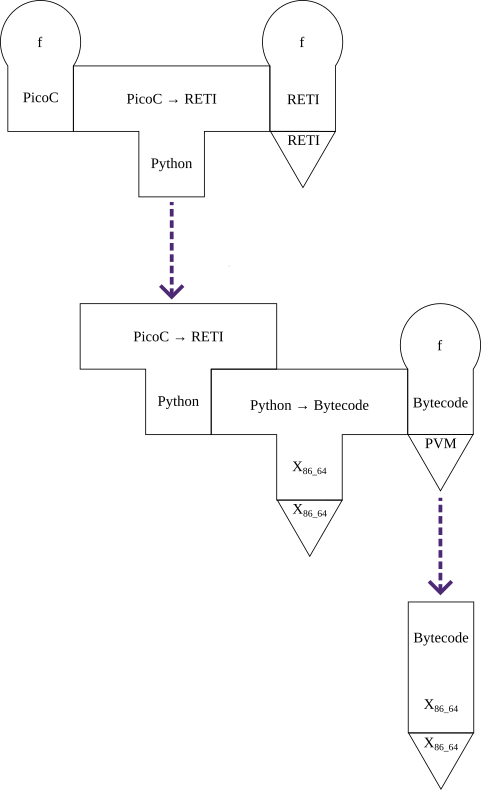
\includegraphics[width=0.5\linewidth]{./figures/summarized_cross_compiler.png}
  \caption{Cross-Compiler Kompiliervorgang ausgeschrieben}
  \label{fig:cross_compiler_kompiliervorgang_ausgeschrieben}
\end{figure}

Dieses längliche \colorbold{T-Diagram} in Abbildung~\ref{fig:cross_compiler_kompiliervorgang_ausgeschrieben} lässt sich zusammenfassen, sodass man das \colorbold{T-Diagram} in Abbildung~\ref{fig:cross_compiler_kompiliervorgang_kurzform} erhält, in welcher direkt angegeben ist, dass der \colorbold{PicoC-Compiler} in $\mathtt{X_{86\_64}}$-Maschienensprache geschrieben ist.

\begin{figure}[H]
  \centering
  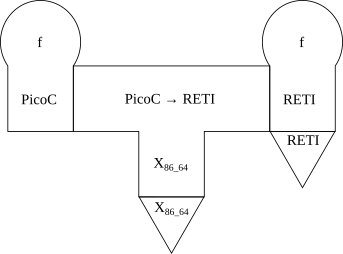
\includegraphics[width=0.33\linewidth]{./figures/compiliervorang_mit_machiene.png}
  \caption{Cross-Compiler Kompiliervorgang Kurzform}
  \label{fig:cross_compiler_kompiliervorgang_kurzform}
\end{figure}

Nachdem der Kompilierprozess des \colorbold{PicoC-Compiler} im \colorbold{vertikalen} nun genauer angesehen wurde, wird der Kompilierprozess im Folgenden im \colorbold{horinzontalen}, auf der Ebene der verschiedenen \colorbold{Passes} genauer betrachtet. Die Abbildung~\ref{fig:architektur_mit_allen_passes_ausgeschrieben} gibt einen guten Überblick über alle \colorbold{Passes} und wie diese in der \colorbold{Pipe-Architektur} (Definition~\ref{def:pipe_architektur}) des \colorbold{PicoC-Compilers} aufeinanderfolgen. In der \colorbold{Pipe-Architektur} nutzt der jeweils nächste \colorbold{Pass} den generierten \colorbold{Abstract Syntax Tree} des vorherigen Passes oder der Syntaktischen Analyse, um einen eigenen \colorbold{Abstract Syntax Tree} in seiner eigenen \colorbold{Sprache} zu generieren.

\begin{figure}[H]
  \centering
  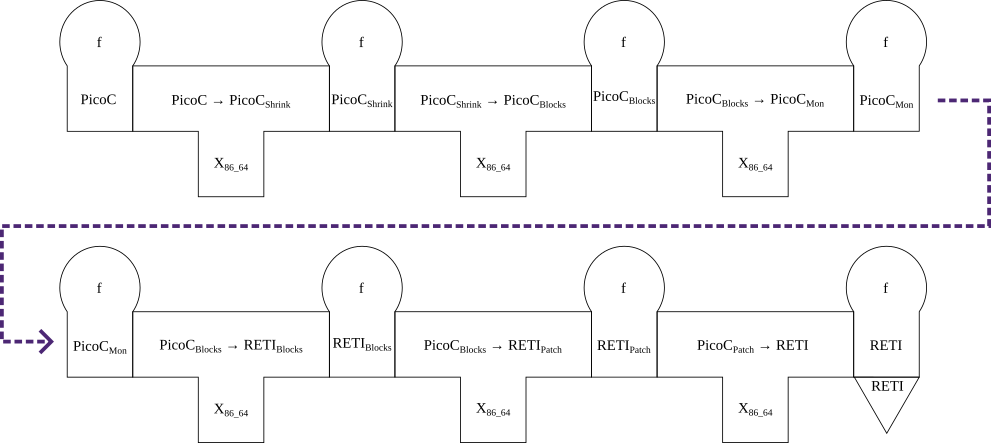
\includegraphics[width=\linewidth]{./figures/passes.png}
  \caption{Architektur mit allen Passes ausgeschrieben}
  \label{fig:architektur_mit_allen_passes_ausgeschrieben}
\end{figure}

Im Unterkapitel~\ref{sec:passes} werden die unterschiedlichen \colorbold{Passes} des PicoC-Compilers erklärt. In den darauffolgenden Unterkapiteln~\ref{sec:umsetzung_von_pointern},~\ref{sec:umsetzung_von_arrays},~\ref{sec:umsetzung_von_structs}~und~\ref{sec:umsetzung_von_funktionen} zu \colorbold{Pointern},  \colorbold{Arrays}, \colorbold{Structs} und \colorbold{Funktionen} werden einzelne \colorbold{Aspekte}, die Thema dieser \colorbold{Bachelorarbeit} sind \colorbold{genauer betrachtet} und erklärt, die im Unterkapitel~\ref{sec:passes} nicht ausreichend vertieft wurden. Viele der verwendenten \colorbold{Ansätze} zur Lösung dieser Probleme basieren auf der Vorlesung~\cite{scholl_betriebssysteme_2020} und wurden in dieser Bachelorarbeit weiter ausgearbeitet, wo es nötig war, sodass diese mit dem \colorbold{PicoC-Compiler} auch in der \colorbold{Praxis} implementiert werden konnten.

% https://tex.stackexchange.com/questions/167380/how-to-refer-to-a-footnote
Um die verschiedenen Aspekte besser erklären zu können, werden \colorbold{Codebeispiele} verwendet, in welchen ein kleines repräsentatives \colorbold{PicoC-Programm} für einen spezifischen Aspekt in wichtigen \colorbold{Zwischenstadien der Kompilierung} gezeigt wird\footnote{Also die verschiedenen in den \colorbold{Passes} generierten \colorbold{Abstract Syntax Trees}, sofern der \colorbold{Pass} für den gezeigten Aspekt relevant ist.}. Die \colorbold{Codebeispiele} wurden alle mit dem \colorbold{PicoC-Compiler} kompiliert und danach \colorbold{nicht} mehr \colorbold{verändert}, also genauso, wie der \colorbold{PicoC-Compiler} sie kompiliert aus den Dateien in dieses Dokument eingelesen. Alle hier zur Repräsentation verwendeten \colorbold{PicoC-Programme} lassen sich unter dem \footnoteurl{https://github.com/matthejue/Bachelorarbeit/tree/master/code_examples} finden und mithilfe der im Ordner \inlinebox{/code_examples} beiliegenden \inlinebox{Makefile} und dem Befehl \inlinebox*{make compile-all} genauso \colorbold{kompilieren}, wie sie hier dargestellt sind\footnote{Es wurden zu diesem Zweck spezielle neue \colorbold{Command-line Optionen} erstellt, die bestimmte Kommentare \colorbold{herausfiltern} und manche Container-Knoten \colorbold{einzeilig} machen, damit die generierten \colorbold{Abstract Syntax Trees} in den verscchiedenen Zwischenstufen der Kompilierung \colorbold{nicht} zu langgestreckt und \colorbold{überfüllt} mit Kommentaren sind.}.

\subsection{Passes}
\label{sec:passes}

Im Folgenden werden die verschiedenen \colorbold{Passes} des \colorbold{PicoC-Compilers} für die Generierung von \colorbold{RETI-Code} besprochen. Viele dieser \colorbold{Passes} haben \colorbold{Aufgaben}, die eher unter die Themenbereiche des \colorbold{Bachelorprojekts} fallen. Allerdings ist das Verständnis der \colorbold{Passes} auch für das Verständnis der veschiedenen Aspekte\footnote{In kurz: \colorbold{Pointer}, \colorbold{Arrays}, \colorbold{Strcuts} und \colorbold{Funktionen}.} der \colorbold{Bachelorarbeit} wichtig.

Auf jedes Detail der einzelnen \colorbold{Passes} wird in diesem Unterkapitel allerdings nicht eingegangen, da diese einerseits in den Unterkapiteln~\ref{sec:umsetzung_von_pointern},~\ref{sec:umsetzung_von_arrays},~\ref{sec:umsetzung_von_structs}~und~\ref{sec:umsetzung_von_funktionen} zu \colorbold{Pointern},  \colorbold{Arrays}, \colorbold{Structs} und \colorbold{Funktionen} im Detail erklärt sind und andererseits viele Aufgaben dieser \colorbold{Passes} eher dem \colorbold{Bachelorprojekt} zuzurechnen sind.

\subsubsection{PicoC-Shrink Pass}
\label{picoc_shrink_pass}
\newlineparagraph{Aufgabe}
\label{sec:picoc_shrink_pass_zweck}
% dieser Pass existiert nur wegen der Erweiterungen

Der Aufgabe des \colorbold{PicoC-Shrink Pass} ist in Unterkapitel~\ref{dereferenzierung_durch_zugriff_auf_arrayindex_ersetzen} ausführlich an einem Beispiel erklärt. Kurzgefasst hat der \colorbold{PicoC-Shrink Pass} die Aufgabe, die Eigenheit auszunutzen, dass der \colorbold{Dereferenzierungoperator} \smalltt{*pntr} und die damit einhergehende \colorbold{Pointer Arithmetik} \smalltt{*(pntr + i)} sich in der Untermenge der Sprache $L_{C}$, welche die Sprache $L_{PicoC}$ darstellt genau gleich verhält, wie der \colorbold{Operator} für den \colorbold{Zugriff} auf den \colorbold{Index} eines \colorbold{Arrays} \smalltt{ar[i]}.

Daher wandelt der \colorbold{PicoC-Shrink Pass} alle Verwendungen des \colorbold{Knoten} \smalltt{Deref(exp, i)} im jeweiligen \colorbold{Abstract Syntax Tree} in \colorbold{Knoten} \smalltt{Subscr(exp, i)} um, sodass sich dadurch viele vermeidbare \colorbold{Fallunterscheidungen} und \colorbold{doppelter Code} bei der Implementierung vermeiden lassen. Man lässt die  \colorbold{Derefenzierung} \smalltt{*(var + i)} einfach von den Routinen für einen \colorbold{Zugriff auf einen Arrayindex} \smalltt{var[i]} übernehmen.

\newlineparagraph{Abstrakte Syntax}

Die \colorbold{Abstrakte Syntax} der Sprache $L_{PicoC\_Shrink}$ in Tabelle~\ref{gr:abstract_syntax_l_picoc_shrink} ist fast \colorbold{identisch} mit der \colorbold{Abstrakten Syntax} der Sprache $L_{PiocC}$ in Tabelle~\ref{gr:abstract_syntax_l_picoc}, nach welcher der \colorbold{erste} Abstract Syntax Tree in der \colorbold{Syntaktischen Analyse} generiert wurde. Der einzige \colorbold{Unterschied} liegt darin, dass es den Knoten \smalltt{Deref(exp, exp)} in Tabelle~\ref{gr:abstract_syntax_l_picoc_shrink} \colorbold{nicht} mehr gibt. Das liegt daran, dass dieser Pass alle \colorbold{Vorkommnisse} des Knoten \smalltt{Deref(exp, exp)} durch den Knoten \smalltt{Subscr(exp, exp)} auswechselt, der ebenfalls bereits in der \colorbold{Abstrakten Syntax} der Sprache $L_{PicoC}$ definiert ist.

\begin{grammar}[Abstrakte Syntax der Sprache $L_{PiocC\_Shrink}$][H][gr:abstract_syntax_l_picoc_shrink]
  \toprule
  \commentsecond*
  \midrule
  \arith*
  \midrule
  \logic*
  \midrule
  \assign*
  \midrule
  \pntrshrink*
  \midrule
  \arraysecond*
  \midrule
  \struct*
  \midrule
  \ifelse*
  \midrule
  \loopsecond*
  \midrule
  \fun*
  \midrule
  \file*
  \bottomrule
\end{grammar}

\begin{Special_Paragraph}
  Der \textcolor{red}{rot} markierte Knoten bedeutet, dass dieser im Vergleich zur voherigen \colorbold{Abstrakten Syntax} nicht mehr da ist.
\end{Special_Paragraph}

\newlineparagraph{Codebeispiel}

In den nächsten Unterkapiteln wird das Beispiel in Code~\ref{code:picoc_code_für_codebeispiel} zur \colorbold{Anschauung} der verschiedenen \colorbold{Passes} verwendet. Im Code~\ref{code:picoc_code_für_codebeispiel} ist in der Funktion \smalltt{faculty} ein \colorbold{iterativer} Algorithmus implementiert, der die \colorbold{Fakultät} eines übergebenen \colorbold{Arguments} berechnet. Der Algorithmus basiert auf einem \colorbold{Beispielprogramm} aus der Vorlesung~\cite{scholl_betriebssysteme_2020}, welcher in der Vorlesung allerdings \colorbold{rekursiv} implementiert ist.
% natürlich beide Beispiele als Tests verfügbar

Dieser \colorbold{rekursive} Algoirthmus ist allerdings \colorbold{kein} gutes \colorbold{Anschaungsbeispiel}, dass viele der Aufgaben der verschiedenen \colorbold{Passes} bei der Kompilierung veranschaulicht hätte. Viele Aufgaben der \colorbold{Passes}, wie z.B. bei der Kompilierung von \smalltt{if}-, \smalltt{if-else}-, \smalltt{while}- und \smalltt{do-while}-Statements wären im Beispiel aus der Vorlesung \colorbold{nicht} enthalten gewesen. Daher wurde das Beispiel aus der Vorlesung zu einem \colorbold{iterativen} Algorithmus~\ref{code:picoc_code_für_codebeispiel} umgeschrieben, um \smalltt{if}- und \smalltt{while}-Statemtens zu enthalten.

Beide Varianten des \colorbold{Algorithmus} wurden zum \colorbold{Testen} des PicoC-Compilers verwendet und sind als Tests im Ordner \inlinebox{/tests} unter \footnoteurl{https://github.com/matthejue/PicoC-Compiler/tree/new_architecture/tests}, unter den Testbezeichnungen \inlinebox{example_faculty_rec.picoc} und \inlinebox{example_faculty_it.picoc} zu finden.

Die Codebeispiele in diesem und den folgenden Unterkapiteln dienen allerdings nur als \colorbold{Anschauung} des jeweiligen \colorbold{Passes}, der in diesem Unterkapitel beschrieben wird und werden nicht im Detail erläutert, da viele Details der Passes später in den Unterkapiteln~\ref{sec:umsetzung_von_pointern},~\ref{sec:umsetzung_von_arrays},~\ref{sec:umsetzung_von_structs}~und~\ref{sec:umsetzung_von_funktionen} zu \colorbold{Pointern},  \colorbold{Arrays}, \colorbold{Structs} und \colorbold{Funktionen} mit eigenen \colorbold{Codebeispielen} erklärt werden und alle sonstigen Details dem \colorbold{Bachelorprojekt} zuzurechnen sind.

\begin{code}
  \centering
  \numberedcodebox[minted language=c]{./code_examples/example_faculty_it.picoc}
  \caption{PicoC Code für Codebespiel}
  \label{code:picoc_code_für_codebeispiel}
\end{code}

In Code~\ref{code:abstract_syntax_tree_für_codebeispiel} sieht man den \colorbold{Abstract Syntax Tree}, der in der \colorbold{Syntaktischen Analyse} generiert wurde.

\begin{code}
  \centering
  \numberedcodebox[minted language=text]{./code_examples/example_faculty_it.ast}
  \caption{Abstract Syntax Tree für Codebespiel}
  \label{code:abstract_syntax_tree_für_codebeispiel}
\end{code}

Im \colorbold{PicoC-Shrink-Pass} ändert sich nichts im Vergleich zum \colorbold{Abstract Syntax Tree} in Code~\ref{code:abstract_syntax_tree_für_codebeispiel}, da das Codebeispiel keine \colorbold{Dereferenzierung} enthält.

% TODO: nichts hinzugefügt zu Syntax

\subsubsection{PicoC-Blocks Pass}
\label{picoc_blocks_pass}
\newlineparagraph{Aufgabe}
\label{sec:picoc_blocks_pass_zweck}

Die Aufgabe des \colorbold{PicoC-Blocks Passes} ist es die Knoten \smalltt{If(exp, stmts)}, \smalltt{IfElse(exp, stmts1, stmts2)}, \smalltt{While(exp, stmts)} und \smalltt{DoWhile(exp, stmts)} mithilfe von \smalltt{Block(name, stmts\_instrs}-, \smalltt{GoTo(lable)}- und \smalltt{IfElse(exp, stmts1, stmts2)}-Knoten umzusetzen. Der \smalltt{IfElse(exp, stmts1, stmts2)}-Knoten wird zur Umsetzung der \colorbold{Bedingung} verwendet und es wird, je nachdem, ob die Bedingung \colorbold{wahr} oder \colorbold{falsch} ist mithilfe der \smalltt{GoTo(label)}-Knoten in einen von zwei \colorbold{alternativen Branches} gesprungen oder ein \colorbold{Branch} erneut aufgerufen usw.

\newlineparagraph{Abstrakte Syntax}

Zur Umsetzung dieses Passes ist es notwendig die \colorbold{Abstrakte Syntax} der Sprache $L_{PicoC\_Shrink}$ in Tabelle~\ref{gr:abstract_syntax_l_picoc_shrink} um die Knoten zu erweitern, die im Unterkapitel \ref{sec:picoc_blocks_pass_zweck} erwähnt wurden. Die Knoten \smalltt{If(exp, stmts)}, \smalltt{While(exp, stmts)} und \smalltt{DoWhile(exp, stmts)} gibt es nicht mehr, da sie durch \smalltt{Block(name, stmts\_instrs}-, \smalltt{GoTo(lable)}- und \smalltt{IfElse(exp, stmts1, stmts2)}-Knoten ersetzt wurden. Die \colorbold{Funktionsdefinition} \smalltt{FunDef(⟨datatype⟩, Name(str), Alloc(Writeable(), ⟨datatype⟩, Name(str))*, ⟨block⟩*)} ist nun ein Container für \colorbold{Blöcke} \smalltt{Block(Name(str), ⟨stmt⟩*)} und keine Statements \smalltt{stmt} mehr. Das resultiert in der \colorbold{Abstrakten Syntax} der Sprache $L_{PicoC\_Blocks}$ in Tabelle~\ref{gr:abstract_syntax_l_picoc_blocks}.

\begin{grammar}[Abstrakte Syntax der Sprache $L_{PiocC\_Blocks}$][H][gr:abstract_syntax_l_picoc_blocks]
  \toprule
  \commentsecond*
  \midrule
  \arith*
  \midrule
  \logic*
  \midrule
  \assign*
  \midrule
  \pntrshrinkafter*
  \midrule
  \arraysecond*
  \midrule
  \struct*
  \midrule
  \ifelseblocks*
  \midrule
  \loopblocks*
  \midrule
  \funafter*
  \midrule
  \block
  \midrule
  \file*
  \bottomrule
\end{grammar}

\begin{Special_Paragraph}
  Alles \textcolor{red}{rot} markierte bedeutet, es wurde \colorbold{entfernt} oder \colorbold{abgeändert}. Alles \textcolor{gray!90!black}{ausgegraute} bedeutet, es hat sich im Vergleich zur letzten Abstrakten Syntax \colorbold{nichts} geändert. Alle normal in \smalltt{schwarz} geschriebenen Knoten wurden \colorbold{neu} hinzugefügt.

  Die \colorbold{Abstrakte Syntax} soll im Gegensatz zur \colorbold{Konkretten Syntax} meist nur vom \colorbold{Programmierer} verstanden werden, der den Compiler implementiert und sollte daher vor allem \colorbold{einfach verständlich} sein und stellt daher eine \colorbold{Obermenge} aller tatsächlich möglichen \colorbold{Kompositionen} von \colorbold{Knoten} dar\footnote{D.h. auch wenn dort \smalltt{exp} als \colorbold{Attribut} steht, kann dort \colorbold{nicht} jeder Knoten, der sich aus der \colorbold{Produktion} \smalltt{exp} ergibt auch wirklich eingesetzt werden.}.

  Man bezeichnet hier die \colorbold{Abstrakte Syntax} als \colorbold{\enquote{Abstrakte Syntax der Sprache $L_{Picoc\_Blocks}$}}. Diese Sprache $L_{Picoc\_Blocks}$ wird durch eine \colorbold{Konkrette Syntax} beschrieben, die allerdings nicht weiter relevant ist, da in den \colorbold{Passes} nur \colorbold{Abstract Syntax Trees} umgeformt werden. Es ist hierbei nur wichtig zu wissen, dass die \colorbold{Abstrakte Syntax} theoretisch zur Kompilierung der Sprache $L_{Picoc\_Blocks}$ definiert ist, also die Sprache $L_{PicoC\_Blocks}$ nicht die Sprache ist, die von der \colorbold{Abstrakten Syntax} beschrieben ist.
\end{Special_Paragraph}
% TODO: man tut so als gäbe es Konkrette Syntax

\newlineparagraph{Codebeispiel}

In Code~\ref{code:picoc_blocks_pass_für_codebeispiel} sieht man den \colorbold{Abstract-Syntax-Tree} des \colorbold{PiocC-Blocks Passes} für das aus Unterkapitel~\ref{code:picoc_code_für_codebeispiel} weitergeführte Beispiel, indem nun eigene \colorbold{Blöcke} für die Funktion \smalltt{faculty} und die \smalltt{main}-Funktion erstellt werden, in denen die \colorbold{ersten} Statements der jeweiligen Funktionen bis zum \colorbold{letzten} Statement oder bis zum ersten \colorbold{Auftauchen} eines \smalltt{If(exp, stmts)}-, \smalltt{IfElse(exp, stmts1, stmts2)}-, \smalltt{While(exp, stmts)}- oder \smalltt{DoWhile(exp, stmts)}-Knoten stehen. Je nachdem, ob ein \smalltt{If(exp, stmts)}-, \smalltt{IfElse(exp, stmts1, stmts2)}-, \smalltt{While(exp, stmts)}- oder \smalltt{DoWhile(exp, stmts)}-Knoten auftaucht, werden für die \colorbold{Bedingung} und mögliche \colorbold{Branches} eigene \colorbold{Blöcke} erstellt.

\begin{code}
  \centering
  \numberedcodebox[minted language=text]{./code_examples/example_faculty_it.picoc_blocks}
  \caption{PicoC-Blocks Pass für Codebespiel}
  \label{code:picoc_blocks_pass_für_codebeispiel}
\end{code}

\subsubsection{PicoC-ANF Pass}
\label{picoc_mon_pass}

\newlineparagraph{Aufgabe}
\label{sec:picoc_mon_pass_zweck}

Die Aufgabe des \colorbold{PicoC-ANF Passes} ist es den \colorbold{Abstract Syntax Tree} der Sprache $L_{PicoC\_Blocks}$ in die \colorbold{Abstrakte Syntax} der Sprache $L_{PicoC\_ANF}$ umzuformen, welche in \colorbold{A-Normalform} (Definition~\ref{def:a_normal_form}) und damit auch in \colorbold{Monadischer Normalform} (Definition~\ref{def:monadische_normalform}) ist. Um Wiederholung zu vermeiden wird zur Erklärung der \colorbold{A-Normalform} auf Unterkapitel~\ref{sec:a_normalform} verwiesen.

Zudem wird eine \colorbold{Symboltabelle} (Definition~\ref{def:symboltabelle}) eingeführt. In der \colorbold{Symboltabelle} wird beim Anlegen eines \colorbold{neuen Eintrags} für eine Variable zunächst eine \colorbold{Adresse} zugewiesen, die dem Wert einer von zwei \colorbold{Countern}  \smalltt{rel\_global\_addr} und  \smalltt{rel\_stack\_addr} entspricht. Der Counter \smalltt{rel\_global\_addr} ist für Variablen in den \colorbold{Globalen Statischen Daten} und der \colorbold{Counter}  \smalltt{rel\_stack\_addr} ist für Variablen auf dem \colorbold{Stackframe}. Einer der beiden \colorbold{Counter} wird entsprechend der \colorbold{Größe} der angelegten Variable \colorbold{hochgezählt}.

Kommt im \colorbold{Programmcode} an einer späteren Stelle diese Variable \smalltt{Name('symbol')} vor, so wird mit dem \colorbold{Symbol}\footnote{Bzw. der \colorbold{Bezeichner}} als Schlüssel in der \colorbold{Symboltabelle} nachgeschlagen und anstelle des \smalltt{Name(str)}-Knotens die in der \colorbold{Symboltabelle} nachgeschlagene Adresse in einem \smalltt{Global(Num('addr'))}- bzw. \smalltt{Stackframe(Num('addr'))}-Knoten eingesetzt eingefügt. Ob der \smalltt{Global(Num('addr'))}- oder  der \smalltt{Stackframe(Num('addr'))}-Knoten zum Einsatz kommt, entscheidet sich anhand des \colorbold{Scopes} (z.B. \smalltt{@scope}), der in der \colorbold{Symboltabelle} an den \colorbold{Bezeichner} drangehängt ist (z.B. \smalltt{identifier@scope}).\footnote{Die Umsetzung von \colorbold{Scopes} wird in Unterkapitel~\ref{sec:funktionsdeklaration_und_definition_und_umsetzung_von_scopes} genauer beschrieben.}

\begin{Definition}{Symboltabelle}{symboltabelle}
  Eine über ein \colorbold{Assoziatives Feld} umgesetzte \colorbold{Datenstruktur}, die notwendig ist, um das Konzept einer \colorbold{Variablen} in einer Sprache umzusetzen. Diese Datenstruktur ordnet jedem \colorbold{Symbol}\footnote{In einer \colorbold{Symboltabelle} werden \colorbold{Bezeichner} als \colorbold{Symbole} bezeichnet.} einer \colorbold{Variablen}, \colorbold{Konstanten} oder \colorbold{Funktion} aus einem \colorbold{Programm}, Informationen, wie die \colorbold{Adresse}, die \colorbold{Position} im Programmcode oder den \colorbold{Datentyp} zu.

  Die \colorbold{Symboltabelle} muss nur während des \colorbold{Kompiliervorgangs} im \colorbold{Speicher} existieren, da die Einträge in der \colorbold{Symboltabelle} beeinflussen, was für \colorbold{Maschinencode} generiert wird und dadurch im \colorbold{Maschinencode} bereits die richtigen \colorbold{Adressen} usw. angesprochen werden und es die Symboltabelle selbst \colorbold{nicht} mehr braucht.
\end{Definition}

\newlineparagraph{Abstrakte Syntax}

Zur Umsetzung dieses Passes ist es notwendig die \colorbold{Abstrakte Syntax} der Sprache $L_{PicoC\_Blocks}$ in Tabelle~\ref{gr:abstract_syntax_l_picoc_blocks} in die \colorbold{A-Normalform} zu bringen. Darunter fällt es unter anderem, dafür zu sorgen, dass \colorbold{Komplexe Knoten}, wie z.B. \smalltt{BinOp(exp, bin\_op, exp)} nur \colorbold{Atomare Knoten}, wie z.B. \smalltt{Stack(Num(str))} enthalten können. Des Weiteren werden auch \colorbold{Funktionen} und \colorbold{Funktionsaufrufe} aufgelöst, sodass u.a. die \colorbold{Blöcke} \smalltt{Block(Name(str), stmt*)} nun direkt im \smalltt{File(Name(str), block*)}-Knoten liegen usw., was in Unterkapitel~\ref{sec:umsetzung_von_funktionen} genauer erklärt wird. Die \colorbold{Symboltabelle} ist ebenfalls als \colorbold{Abstract Syntax Tree} umgesetzt, wofür in der \colorbold{Abstrakten Syntax} der Sprache $L_{PicoC\_ANF}$ in Grammatik~\ref{gr:abstract_syntax_l_picoc_anf} neue Knoten eingeführt werden.

Das ganze resultiert in der \colorbold{Abstrakten Syntax} der Sprache $L_{PicoC\_ANF}$ in Grammatik~\ref{gr:abstract_syntax_l_picoc_anf}.

\begin{grammar}[Abstrakte Syntax der Sprache $L_{PiocC\_ANF}$][H][gr:abstract_syntax_l_picoc_anf]
  \toprule
  \commentsecond*
  \midrule
  \arithanf
  \midrule
  \logicanf
  \midrule
  \assignanf
  \midrule
  \pntranf*
  \midrule
  \arrayanf*
  \midrule
  \struct*
  \midrule
  \ifelseanf*
  \midrule
  \funanf*
  \midrule
  \block*
  \midrule
  \fileanf*
  \midrule
  \symbolsecond
  \bottomrule
\end{grammar}

\newlineparagraph{Codebeispiel}

In Code~\ref{code:picoc_mon_pass_für_codebeispiel} sieht man den \colorbold{Abstract-Syntax-Tree} des \colorbold{PiocC-ANF Passes} für das aus Unterkapitel~\ref{code:picoc_code_für_codebeispiel} weitergeführte Beispiel, indem alls Statements und Ausdrücke in \colorbold{A-Normalform} sind. Die \smalltt{IfElse(exp, stmts, stmts)}-Knoten sind hier in  \colorbold{A-Normalform} gebracht worden, indem ihre \colorbold{Komplexe Bedingung} vorgezogen wurde und das Ergebnis der \colorbold{Komplexen Bedingung} einer \colorbold{Location} zugewiesen ist und sie selbst das Ergebnis über den \colorbold{Atomaren Ausdruck} \smalltt{Stack(Num(str))} vom Stack lesen: \smalltt{IfElse(Stack(Num(str)), stmts, stmts)}. \colorbold{Funktionen} sind nur noch über die \colorbold{Labels} von Blöcken zu erkennen, die den gleichen Bezeichner haben, wie die ursprüngliche Funktion und es lässt sich nur durch das \colorbold{Nachverfolgen} der \smalltt{GoTo(Name('label'))}-Knoten nachvollziehen, was ursprünglich zur Funktion gehörte.

\begin{code}
  \centering
  \numberedcodebox[minted language=text]{./code_examples/example_faculty_it.picoc_mon}
  \caption{PicoC-ANF Pass für Codebespiel}
  \label{code:picoc_mon_pass_für_codebeispiel}
\end{code}

\subsubsection{RETI-Blocks Pass}
\label{reti_blocks_pass}

\newlineparagraph{Aufgabe}
\label{sec:reti_blocks_pass_zweck}

Die Aufgabe des \colorbold{RETI-Blocks Passes} ist es die \colorbold{Statements} in der \colorbold{Blöcken}, die durch \colorbold{PicoC-Knoten} im \colorbold{Abstract Syntax Tree} der Sprache $L_{PicoC\_ANF}$ dargestellt sind durch ihren entsprechenden \colorbold{RETI-Knoten} zu ersetzen.

\newlineparagraph{Abstrakte Syntax}

Die \colorbold{Abstrakte Syntax} der Sprache $L_{RETI\_Blocks}$ in Grammatik~\ref{gr:abstract_syntax_l_reti_blocks} ist verglichen mit der \colorbold{Abstrakten Syntax} der Sprache $L_{PicoC\_ANF}$ in Grammatik~\ref{gr:abstract_syntax_l_picoc_anf} stark verändert, denn der Großteil der \colorbold{PicoC-Knoten} wird in diesem Pass durch entsprechende \colorbold{RETI-Knoten} ersetzt. Die einzigen verbleibenden \colorbold{PicoC-Knoten} sind \smalltt{Exp(GoTo(str))}, \smalltt{Block(Name(str), ⟨instr⟩*)} und \smalltt{File(Name(str), ⟨block⟩*)}, da das gesamte Konzept mit den \colorbold{Blöcken} erst im \colorbold{RETI-Pass} in Unterkapitel~\ref{gr:abstract_syntax_l_reti} aufgelöst wird.

\begin{grammar}[Abstrakte Syntax der Sprache $L_{RETI\_Blocks}$][H][gr:abstract_syntax_l_reti_blocks]
  \toprule
  \retiblocks
  \midrule
  \picocblocksleftover
  \bottomrule
\end{grammar}

\newlineparagraph{Codebeispiel}

In Code~\ref{code:reti_blocks_pass_für_codebeispiel} sieht man den \colorbold{Abstract-Syntax-Tree} des \colorbold{RETI-Blocks Passes} für das aus Unterkapitel~\ref{code:picoc_code_für_codebeispiel} weitergeführte Beispiel, indem die \colorbold{Statements}, die durch entsprechende \colorbold{PicoC-Knoten} im \colorbold{Abstrakt Syntax Tree} der Sprache $L_{PicoC\_ANF}$ in Grammatik~\ref{gr:abstract_syntax_l_picoc_anf} repräsentiert waren nun durch ihre entsprechennden \colorbold{RETI-Knoten} ersetzt werden.

\begin{code}
  \centering
  \numberedcodebox[minted language=text]{./code_examples/example_faculty_it.reti_blocks}
  \caption{RETI-Blocks Pass für Codebespiel}
  \label{code:reti_blocks_pass_für_codebeispiel}
\end{code}

\begin{Special_Paragraph}
  Wenn der \colorbold{Abstract Syntax Tree} ausgegeben wird, ist die Darstellung nicht auschließlich in \colorbold{Abstrakter Syntax}, da die \colorbold{RETI-Knoten} aus bereits im Unterkapitel~\ref{sec:ausgabe_von_abstract_syntax_trees} vermitteltem Grund in \colorbold{Konkretter Syntax} ausgeben werden.
\end{Special_Paragraph}

\subsubsection{RETI-Patch Pass}
\label{reti_patch_pass}

\newlineparagraph{Aufgabe}
\label{sec:reti_patch_pass_zweck}

Die Aufgabe des \colorbold{RETI-Patch Passes} ist das \colorbold{Ausbessern} (engl. to patch) des \colorbold{Abstract Syntax Trees}, durch:
\begin{itemize}
  \item das \colorbold{Einfügen} eines \smalltt{start.<nummer>}-Blockes, welcher ein \smalltt{GoTo(Name('main'))} zur  \smalltt{main}-Funktion enthält, wenn in manchen Fällen die \smalltt{main}-Funktion \colorbold{nicht} die erste Funktion ist und daher am Anfang zur \smalltt{main}-Funktion gesprungen werden muss.
  \item das \colorbold{Entfernen} von \smalltt{GoTo()}'s, deren Sprung nur \colorbold{eine} Adresse weiterspringen würde.
  \item das \colorbold{Voranstellen} von \colorbold{RETI-Knoten}, die vor jeder \colorbold{Division} \smalltt{Instr(Div(), args)} prüfen, ob, nicht durch \smalltt{0} geteilt wird.\footnote{Das fällt unter die Themenbereiche des \colorbold{Bachelorprojekts} und wird daher \colorbold{nicht} genauer erläutert.}
  \item das Überprüfen darauf, ob bestimmte \colorbold{Immediates} \smalltt{Im(str)} in Befehlen, wie z.B. \smalltt{Jump(rel, Im(str))}, \smalltt{Instr(Loadin(), [reg, reg, Im(str)])}, \smalltt{Instr(Loadi(), [reg, Im(str)])} usw. \colorbold{kleiner} $-2^{21}$ oder \colorbold{größer} $2^{21}-1$ sind. Im Fall dessen, dass es so ist, muss der \colorbold{gewünschte Zahlenwert} durch \colorbold{Bitshiften} und Anwenden von \colorbold{bitweise Oder} berechnet werden. Im Fall, dessen, dass der \colorbold{Immediate} allerdings \colorbold{kleiner} $-(2^{31})$ oder \colorbold{größer} $2^{31} - 1$ ist, wird eine Fehlermeldung \smalltt{TooLargeLiteral} ausgegeben.
\end{itemize}

\newlineparagraph{Abstrakte Syntax}

Die \colorbold{Abstrakte Syntax} der Sprache $L_{RETI\_Patch}$ in Grammatik~\ref{gr:abstract_syntax_l_reti_patch} ist im Vergleich zur \colorbold{Abstrakten Syntax} der Sprache $L_{RETI\_Blocks}$ in Grammatik~\ref{gr:abstract_syntax_l_reti_blocks} kaum verändert. Es muss nur ein Knoten \smalltt{Exit()} hinzugefügt werden, der im Falle einer  \colorbold{Division durch $0$} die Ausführung des Programs beendet.

\begin{grammar}[Abstrakte Syntax der Sprache $L_{RETI\_Patch}$][H][gr:abstract_syntax_l_reti_patch]
  \toprule
  \retiblocks*
  \midrule
  \picocblocksleftover*
  \bottomrule
\end{grammar}

\newlineparagraph{Codebeispiel}

In Code~\ref{code:reti_patch_pass_für_codebeispiel} sieht man den \colorbold{Abstract-Syntax-Tree} des \colorbold{PiocC-Patch Passes} für das aus Unterkapitel~\ref{code:picoc_code_für_codebeispiel} weitergeführte Beispiel. Durch den \colorbold{RETI-Patch Pass} wurde hier ein \smalltt{start.<nummer>}-Block\footnote{Dieser \colorbold{Block} wurde im Code~\ref{code:picoc_blocks_pass_für_codebeispiel} markiert.} eingesetzt, da die \smalltt{main}-Funktion \colorbold{nicht} die \colorbold{erste} Funktion ist. Des Weiteren wurden durch diesen Pass einzelne \smalltt{GoTo(Name(str))}-\colorbold{Statements} entfernt\footnote{Diese \colorbold{entfernten} \smalltt{GoTo(Name(str))}'s' wurden ebenfalls im Code~\ref{code:picoc_blocks_pass_für_codebeispiel} markiert.}, die nur einen Sprung um \colorbold{eine} Position entsprochen hätten.

\begin{code}
  \centering
  \numberedcodebox[minted language=text, minted options={highlightlines={4-9,24,38,66}}]{./code_examples/example_faculty_it.reti_patch}
  \caption{RETI-Patch Pass für Codebespiel}
  \label{code:reti_patch_pass_für_codebeispiel}
\end{code}

\subsubsection{RETI Pass}
\label{reti_pass}

\newlineparagraph{Aufgabe}
\label{sec:reti_pass_zweck}

Die Aufgabe des \colorbold{RETI-Patch Passes} ist es die \smalltt{GoTo(Name(str))}-Knoten in den den Knoten \smalltt{Instr(Loadi(), [reg, GoTo(Name(str))])}, \smalltt{Jump(Eq(), GoTo(Name(str)))} und \smalltt{Exp(GoTo(Name(str)))} durch eine entsprechende \colorbold{Adresse} zu ersetzen, die entsprechende \colorbold{Distanz} oder einen entsprechenden \colorbold{Sprungbefehl} mit passender \colorbold{Distanz} \smalltt{Jump(Always(), Im(str(distance)))}. Die \colorbold{Distanz-} und \colorbold{Adressberechnung} wird in Unterkapitel~\ref{sec:funktionsaufruf} genauer mit \colorbold{Formeln} erklärt.

\newlineparagraph{Konkrette und Abstrakte Syntax}

Die \colorbold{Abstrakte Syntax} der Sprache $L_{RETI}$ in Grammatik~\ref{gr:abstract_syntax_l_reti} hat im Vergleich zur \colorbold{Abstrakten Syntax} der Sprache $L_{RETI\_Patch}$ in Grammatik~\ref{gr:abstract_syntax_l_reti_patch} nur noch auschließlich \colorbold{RETI-Knoten}. Alle \colorbold{RETI-Knoten} stehen nun einem \smalltt{Program(Name(str), instr)}-Knoten.

Ausgegeben wird der finale \colorbold{Maschinencode} allerdings in \colorbold{Konkretter Syntax}, die sich aus den Grammatiken~\ref{gr:konkrette_syntax_l_reti_lexer} und \ref{gr:konkrette_syntax_l_reti_parser} für jeweils die \colorbold{Lexikalische} und \colorbold{Syntaktische Analyse} zusammensetzt. Der Grund, warum die \colorbold{Konkrette Syntax} der Sprache  $L_{RETI}$ auch nochmal in einen Teil für die \colorbold{Lexikalische} und \colorbold{Syntaktische Analyse} unterteilt ist, hat den Grund, dass für die Bachelorarbeit zum \colorbold{Testen} des \colorbold{PicoC-Compilers} ein \colorbold{RETI-Interpreter} implementiert wurde, der den RETI-Code \colorbold{lexen} und \colorbold{parsen} muss, um ihn später \colorbold{interpretieren} zu können.

% dieser Pass entspricht Assembler bis auf die Sache mit binärer Repräsentation, was der PicoC-Compiler garnicht macht

\begin{grammar}[Konkrette Syntax der Sprache $L_{RETI}$ für die Lexikalische Analyse in EBNF][H][gr:konkrette_syntax_l_reti_lexer]
  \toprule
  \firstcase{dig\_no\_0}{ \dq 1\dq \gralt \dq 2\dq \gralt \dq 3\dq \gralt \dq 4\dq \gralt \dq 5\dq \gralt \dq 6\dq}{L\_Program}
  \otherform{\dq 7\dq \gralt \dq 8\dq \gralt \dq 9\dq}{}
  \firstcase{dig\_with\_0}{ \dq 0\dq \gralt dig\_no\_0}{}
  \firstcase{num}{ \dq 0\dq \gralt dig\_no\_0 \enspace dig\_with\_0*\gralt \dq {-}\dq dig\_no\_0*}{}
  \firstcase{letter}{ \dq a\dq ... \dq Z\dq }{}
  \firstcase{name}{ letter(letter \mid  dig\_with\_0 \mid  \_)*}{}
  \firstcase{reg}{ \dq ACC\dq \gralt \dq IN1\dq \gralt \dq IN2\dq \gralt \dq PC\dq \gralt \dq SP\dq}{}
  \otherform{\dq BAF\dq \gralt \dq CS\dq \gralt \dq DS\dq}{}
  \firstcase{arg}{ reg \gralt  num}{}
  \firstcase{rel}{ \dq {==}\dq \gralt \dq {!=}\dq \gralt \dq {<}\dq \gralt \dq {<=}\dq\gralt \dq {>}\dq}{}
  \otherform{\dq {>=}\dq \gralt \dq \_NOP\dq}{}
  \bottomrule
\end{grammar}

\begin{grammar}[Konkrette Syntax der Sprache $L_{RETI}$ für die Syntaktische Analyse in EBNF][H][gr:konkrette_syntax_l_reti_parser]
\toprule
\firstcase{instr}{\dq ADD\dq\enspace reg\enspace arg\gralt \dq ADDI\dq\enspace reg\enspace num\gralt \dq SUB\dq\enspace reg\enspace arg}{L\_Program}
\otherform{\dq SUBI\dq\enspace reg\enspace\enspace num\gralt \dq MULT\dq\enspace reg\enspace arg\gralt \dq MULTI\dq\enspace reg\enspace num}{}
\otherform{\dq DIV\dq\enspace reg\enspace arg\gralt \dq DIVI\dq\enspace reg\enspace num\gralt \dq MOD\dq\enspace reg\enspace arg}{}
\otherform{\dq MODI\dq\enspace reg\enspace num\gralt \dq OPLUS\dq\enspace reg\enspace arg\gralt \dq OPLUSI\dq\enspace reg\enspace num}{}
\otherform{\dq OR\dq\enspace reg\enspace arg\gralt \dq ORI\dq\enspace reg\enspace num}{}
\otherform{\dq AND\dq\enspace reg\enspace arg\gralt \dq ANDI\dq\enspace reg\enspace num}{}
\otherform{\dq LOAD\dq\enspace reg\enspace num\gralt \dq LOADIN\dq\enspace arg\enspace arg\enspace num}{}
\otherform{\dq LOADI\dq\enspace reg\enspace num}{}
\otherform{\dq STORE\dq\enspace reg\enspace num\gralt \dq STOREIN\dq\enspace arg\enspace arg num}{}
\otherform{\dq MOVE\dq\enspace reg\enspace reg}{}
\otherform{\dq JUMP\dq rel\enspace num\gralt INT\enspace num\gralt RTI}{}
\otherform{\dq CALL\dq\enspace \dq INPUT\dq\enspace  reg\gralt \dq CALL\dq\enspace \dq PRINT\dq\enspace reg}{}
\firstcase{program}{name\enspace (instr\dq ;\dq )*}{}
\bottomrule
\end{grammar}

% TODO: es braucht noch eine Konkrette Syntax dafür
\begin{grammar}[Abstrakte Syntax der Sprache $L_{RETI}$][H][gr:abstract_syntax_l_reti]
  \toprule
  \reti
  \midrule
  \picocremovedleftover
  \bottomrule
\end{grammar}

\newlineparagraph{Codebeispiel}

Nach dem \colorbold{RETI-Pass} ist das Programm komplett in \colorbold{RETI-Knoten} übersetzt, die allerdings in ihrer \colorbold{Konkretten Syntax} ausgegeben werden, wie in Code~\ref{code:reti_pass_für_codebeispiel} zu sehen ist. Es gibt \colorbold{keine Blöcke} mehr und die \colorbold{RETI-Befehle} in diesen Blöcken wurden \colorbold{zusammengesetzt}, wie sie in den \colorbold{Blöcken} angeordnet waren. Die letzten \colorbold{Nicht-RETI-Befehle} oder \colorbold{RETI-Befehle}, die \colorbold{nicht} auschließlich aus \colorbold{RETI-Ausdrücken} bestehen\footnote{Wie z.B. \seqtt{LOADI\; ACC\; GoTo(Name('addr@next\_instr'))}, \seqtt{Exp(GoTo(Name('main.0')))} und \seqtt{JUMP==\; GoTo(Name('if\_else\_after.2'))}.}, die sich in den \colorbold{Blöcken} befunden haben, wurden durch \colorbold{RETI-Befehle} ersetzt.

Der \smalltt{Program(Name(str), instr)}-Knoten, indem alle \colorbold{RETI-Knoten} stehen gibt alleinig die \colorbold{RETI-Knoten}, die er beinhaltet aus und fügt ansonsten nichts hinzu, wodurch der \colorbold{Abstract Syntax Tree}, wenn er in eine Datei ausgegeben wird, direkt \colorbold{RETI-Code} in \colorbold{menschenlesbarer Repräsentation} erzeugt.

\begin{code}
  \centering
  \numberedcodebox[minted language=text]{./code_examples/example_faculty_it.reti}
  \caption{RETI Pass für Codebespiel}
  \label{code:reti_pass_für_codebeispiel}
\end{code}

% TODO: zusammenfassendes Bild
